\chapter{Line-graphes}
\label{linegraphesChapitre}
%--------------------------------------------------------------------
%------- formulation du probleme ---------------------
%--------------------------------------------------------------------
Dans le chapitre pr\'ec\'edent, nous avons d\'etermin\'e la matrice de corr\'elation $M_c$ du graphe $G$ d'un r\'eseau \'electrique. Cette matrice peut contenir des cases \'erron\'ees. Une case \'erron\'ee  $M_c[i,j]$ est un coefficient de corr\'elation proche de $1$ (resp. de $0$) entre les arcs $i$ et $j$ alors que ces arcs ne partagent aucune extr\'emit\'e (resp. ces arcs ont une extr\'emit\'e commune).
\newline
Nous consid\'erons une matrice $M$ de dimension identique \`a celle de $M_c$ telle que, pour toute valeur de seuil $s \in [0,1]$ et toute paire d'arcs $(i,j)$, $M[i,j] = 1$ si et seulement si $M_c[i,j] \ge s$. La matrice $M$ est la matrice d'adjacence d'un graphe non orient\'e $G_c$ dit {\em graphe de corr\'elation}. Cette matrice peut \'egalement contenir des cases \'erron\'ees.  
Une case \'erron\'ee $M[i,j] = 1$ d\'esigne la pr\'esence d'ar\^etes dans $G_c$ alors qu'il n'existe aucune ar\^ete entre les sommets $i$ et $j$ dans le line-grahe du graphe non-orient\'e sous-jacent au DAG $G$. 
De m\^eme, l'absence d'une ar\^ete entre $i$ et $j$ dans $G_c$ alors qu'elle est pr\'esente dans le line-grahe du graphe non-orient\'e sous-jacent \`a $G$ est aussi une case \'erron\'e  $M[i,j] = 0$.
\newline 
S'il n'existe aucune case \'erron\'ee dans la matrice $M$, alors $G_c$ est le line-graphe de graphe non-orient\'e sous-jacent au DAG $G$ et le line-graphe de $G$ est isomorphe \`a $G_c$.
Notre but est de d\'eduire le DAG $G$ \`a partir de $G_c$ en deux \'etapes :
\begin{itemize}
	\item D\'eterminer si $G_c$ est un line-graphe. Si c'est  le cas, d\'eduire le graphe dont $G_c$ est le line-graphe.
	\item Dans le cas o\`u $G_c$ n'est pas un line-graphe, proposer un algorithme qui modifie $G_c$ de telle sorte qu'il devient un line-graphe et ensuite d\'eduire le graphe dont le graphe $G_c$ modifi\'e est le line-graphe.
\end{itemize}
 Nous d\'esignons ce probl\`eme par {\em Proxi-Line}.
\newline
Nous allons, dans un premier temps, d\'ecrire les caract\'eristiques d'un line-graphe et le probl\`eme {\em Proxi-Line}. Ensuite nous pr\'esentons les algorithmes qui traitent ce probl\`eme et enfin nous expliquons la reconstruction de la topologie \`a partir du line-graphe d\'ecouvert par nos algorithmes. 





\section{Line-graphes : caract\'eristiques et propri\'et\'es}
	%------- introduction_line_graphes_caracteristiques ---------
	Dans la th\'eorie des graphes, un line-graphe est aussi appel\'e un {\em graphe adjoint} et ce terme est introduit par l'article de Harary et Norman \cite{harary1960some}.
Le line-graphe d'un graphe non orient\'e $G$ est un graphe qui repr\'esente la relation d'incidence entre les ar\^etes de $G$.
Nous allons d\'efinir formellement le line-graphe d'un graphe et pr\'esenter ses propri\'et\'es.

	
	%------- caracteristiques_linegraphes ----------------
	\subsection{Caract\'eristiques d'un line-graphe}
		
\begin{definition}
\label{definitionLineGraphe}
Soit $G = (V, E)$ un graphe non orient\'e.
\newline
Le line-graphe de $G$ est un graphe non-orient\'e $L(G) = (V',E')$ dans lequel 
$V'=E$ et 
une paire $[a,a']$ de sommets de $L(G)$ est une ar\^ete si et seulement si $a$ et $a'$ ont une extr\'emit\'e commune dans $G$.
\newline
Le graphe $G$ est appel\'e le {\em graphe racine} de $L(G)$.
\end{definition}

Si $G$ est un DAG alors  $L(G)$ est le line-graphe du graphe non-orient\'e sous-jacent \`a $G$.
\'Etant donn\'e que $G$ a $n$ sommets et $m$ arcs (sans arcs sym\'etriques), le graphe $L(G)$ a $m$ sommets et $|E'| = \sum_{i=1 }^{n} d_i(d_i -1)/2$ ar\^etes avec $d_i$ le degr\'e de chaque sommet $i$ de $G$.
\vspace{-0.3cm}

%% ---- figure GrapheRacineLineGrapheExemple
\begin{figure}[htb!]\vspace{-0.5em}
	\centering
	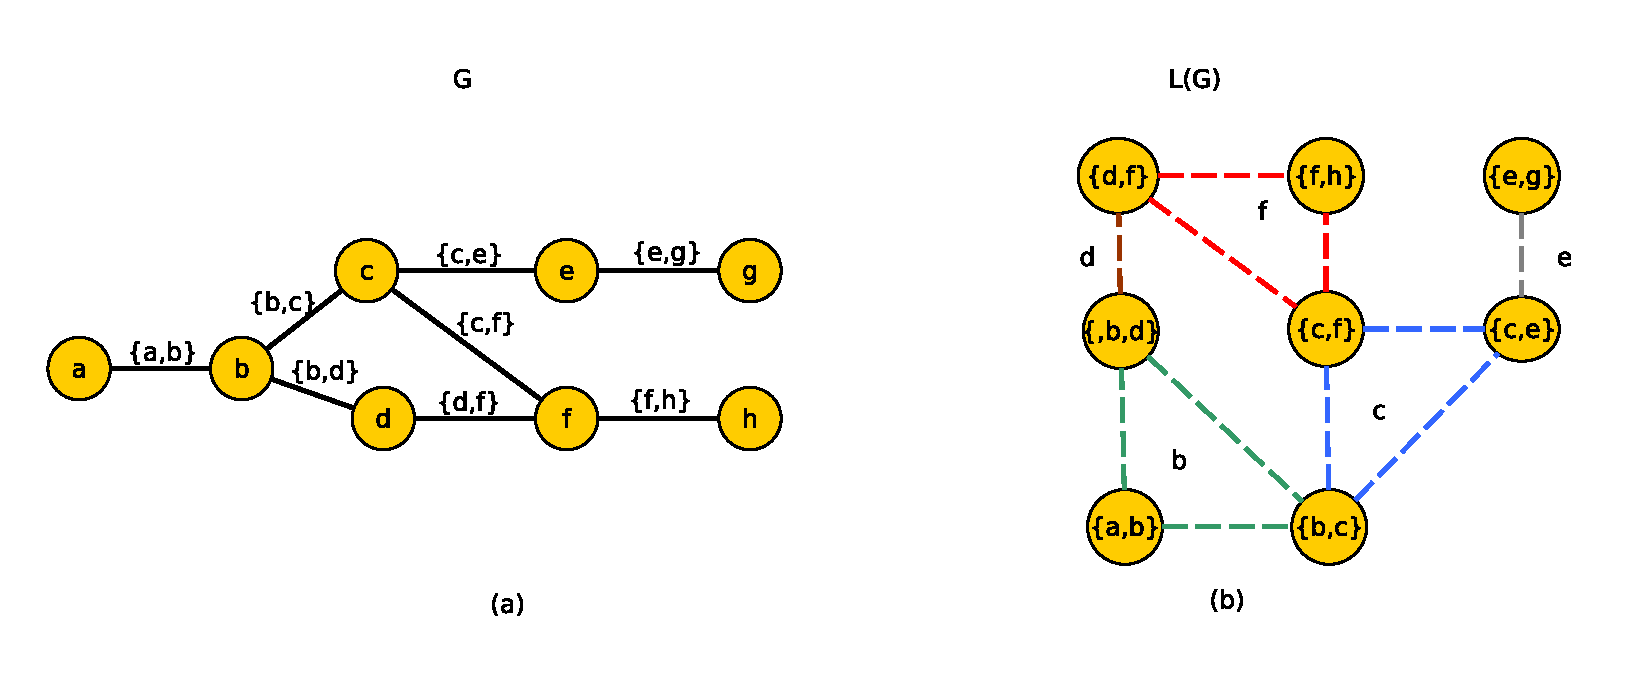
\includegraphics[scale=0.650]{grapheRacineLineGrapheExemple.eps}\vspace{-0.5em}
	\caption{ Le graphe $G$ et son line-graphe $L(G)$. 
			}\vspace{-0.5em}
	\label{grapheRacineLineGrapheExemple}
\end{figure}
%% ---- figure GrapheRacineLineGrapheExemple
\FloatBarrier
\vspace{0.3cm}

La figure \ref{grapheRacineLineGrapheExemple}(a) pr\'esente le graphe $G=(V,E)$ dans lequel l'ensemble $V$ contient $8$ sommets $V=\{a,b,c,d,e,f,g,h\}$ et l'ensemble $E$ contient $8$ ar\^etes \\ $E=\{ \{a,b\}, \{b,c\}, \{b,d\}, \{c,f\}, \{d,f\}, \{f,h\}, \{c,e\},\{e,g\} \}$. 
Chaque ar\^ete de $E$ devient un sommet de $L(G)$ dans la figure \ref{grapheRacineLineGrapheExemple}(b). Lorsque deux ar\^etes de $E$ ont une extr\'emit\'e  commune alors leurs sommets respectifs dans $L(G)$  sont adjacents.
Par exemple, dans la figure \ref{grapheRacineLineGrapheExemple}(b), les sommets $\{b,d\}$ et $\{d,f\}$ sont li\'es par une ar\^ete \`a cause du sommet $d \in V$. 
Nous construisons ainsi le graphe $L(G)$  qui contient $8$ sommets et $11$ ar\^etes.
Nous constatons qu'un sommet de $G$ correspond \`a une clique dans $L(G)$. 
En effet, les sommets de la clique $\{ \{a,b\},  \{b,c\},  \{b,d\} \}$ de taille $3$ dans $L(G)$ concourent \`a un point $b$ de degr\'e $3$ qui est un sommet de $G[V]$. Le sommet  $b$ de $G$  identifie la clique $\{ \{a,b\},  \{b,c\},  \{b,d\} \}$ dans $L(G)$.
Le graphe $L(G)$ est le  line-graphe de $G$ et $G$ est le {\em graphe racine}.
\newline

La notion de {\em line-graphe} a \'et\'e introduite par {\em Whitney} \cite{whitney1932congruent} en se basant sur la notion d'isomorphisme. Il montre que  si deux line-graphes sont isomorphes et connexes alors leurs graphes racines sont aussi isomorphes \`a l'exception des graphes triangle $K_3$ et \'etoile $K_{1,3}$. 
\begin{proposition} \cite{lineGraphe}
Le graphe \'etoile $K_{1,3}$ n'est pas un {\em line-graphe}.
\end{proposition}
\begin{Proof}
{\em
Supposons que $K_{1,3}$ est le line-graphe de $H$ ($K_{1,3} = L(H)$). 
Alors $H$ est un graphe connexe de quatre ar\^etes.
Tous les graphes connexes de quatres ar\^etes sont repr\'esent\'es dans la figure  \ref{graphesRacinesDeQuatresAretes}. 
Comme $L(C_4) = C_4$  et $L(K_{1,3} + e) = K_4 + e$ (voir figure \ref{graphesRacinesDeQuatresAretes}), $L(H)$ ne peut \^etre que l'un des trois arbres $P_4$, $K_{3,2}$ et $K_{1,4}$.
Ce qui est contraire \`a notre hypoth\`ese de d\'epart ($K_{1,3} = L(H)$).}
\end{Proof}
%\newline
% ------ figure graphes Racines De Quatres Aretes
\begin{figure}[htb!]\vspace{-0.5em}
	\centering
	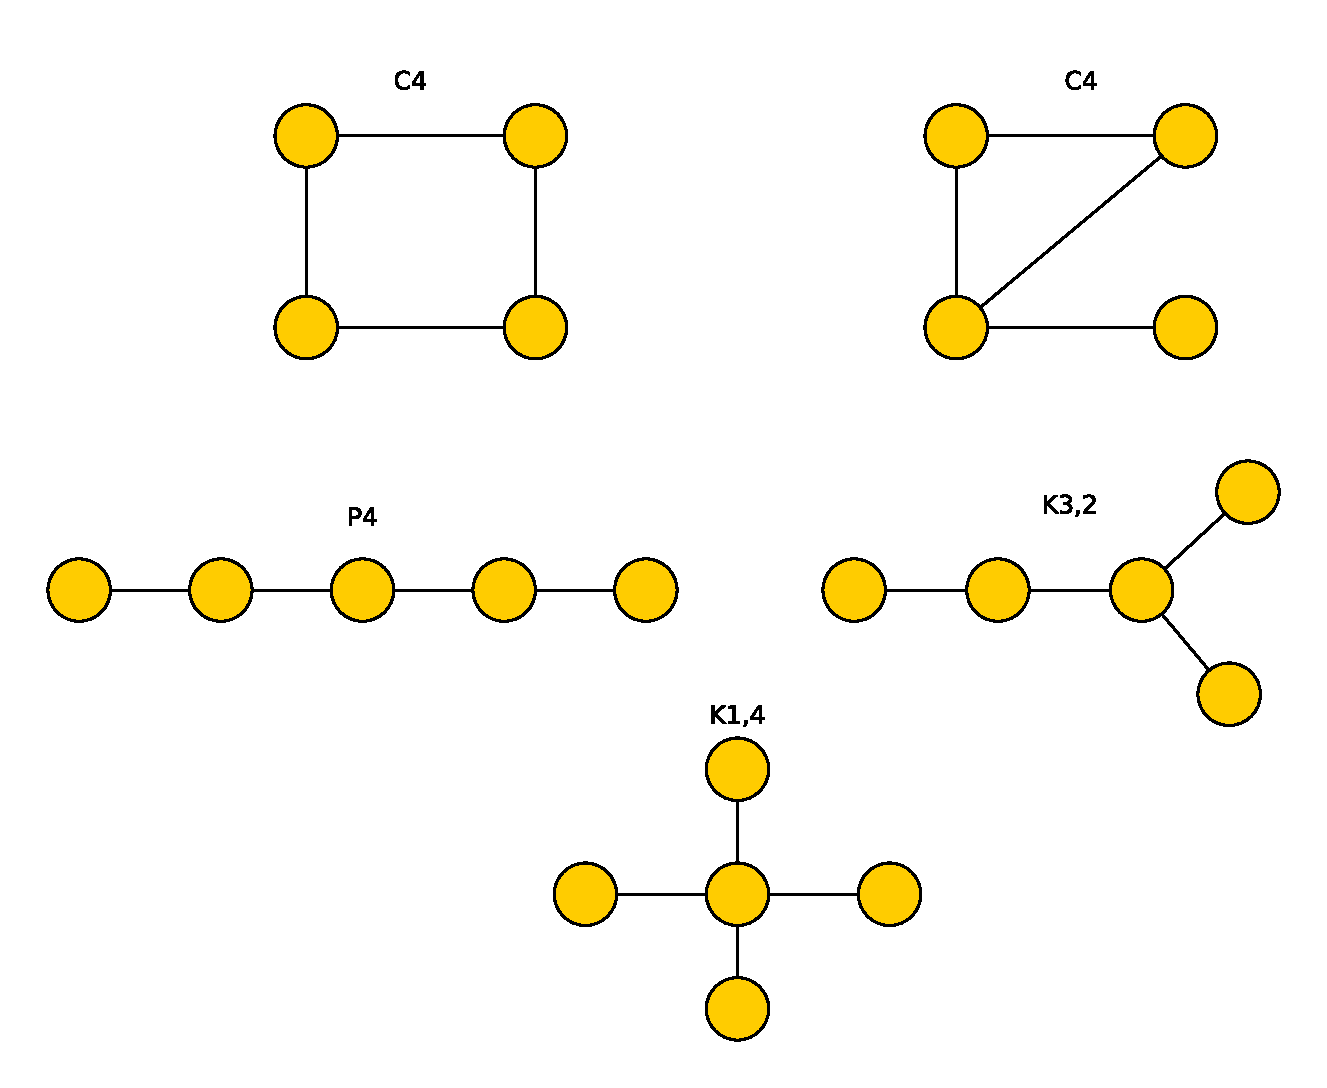
\includegraphics[scale=0.50]{graphesRacinesDeQuatresAretes.eps}\vspace{-0.5em}
	\caption{ Les graphes racines possibles de $K_{1,3}$ de quatres ar\^etes.}\vspace{-0.5em}
	\label{graphesRacinesDeQuatresAretes}
\end{figure}
% ------ figure graphes Racines De Quatres Aretes
\FloatBarrier
\vspace{0.3cm}

Le graphe \'etoile ($K_{1,3}$) a un r\^ole important dans la caract\'erisation des line-graphes.
La premi\`ere caract\'eristique provient des travaux de {\em Krausz} \cite{krausz1943demonstration} et elle est relative au partitionnement du line-graphe en sous-graphes. 
La seconde caract\'eristique, formul\'ee par {\em Van Rooij et Wilf} \cite{ROOIJetWILF1965interchange}, d\'ecrit la structure de base d'un graphe pour \^etre un line-graphe. 
Et enfin, la derni\`ere caract\'eristique pr\'esent\'ee par {\em Beineke\cite{beineke1968derived} et Hemminger} a d\'etermin\'e les neufs sous-graphes ne pouvant pas \^etre les sous-graphes induits  de line-graphes. 
\begin{theorem}\cite{lineGraphe}
\label{caracteristiquesLinegraphes}
Soit $H$ un graphe. Les affirmations suivantes sont \'equivalentes.
\begin{enumerate}[label = (\alph*)]
	\item $H$ est un line-graphe.
	\item Les ar\^etes de $H$ peuvent \^etre partitionn\'ees en sous-graphes complets appel\'es {\em cliques} tel qu'aucun sommet n'est contenu dans plus de deux sous-graphes. 
	\item $H$ ne contient pas $K_{1,3}$ comme sous-graphe et si deux triangles ont une ar\^ete commune alors le sous-graphe induit est $K_4$.
	\item Aucun des neufs sous-graphes de la figure \ref{neufSousGraphesInterditDesLineGraphes} ne peut \^etre un sous-graphe du line-graphe $H$.
\end{enumerate}
\end{theorem}

% ------ figure neuf Sous Graphes Interdit Des LineGraphes
\begin{figure}[htb!]\vspace{-0.5em}
	\centering
	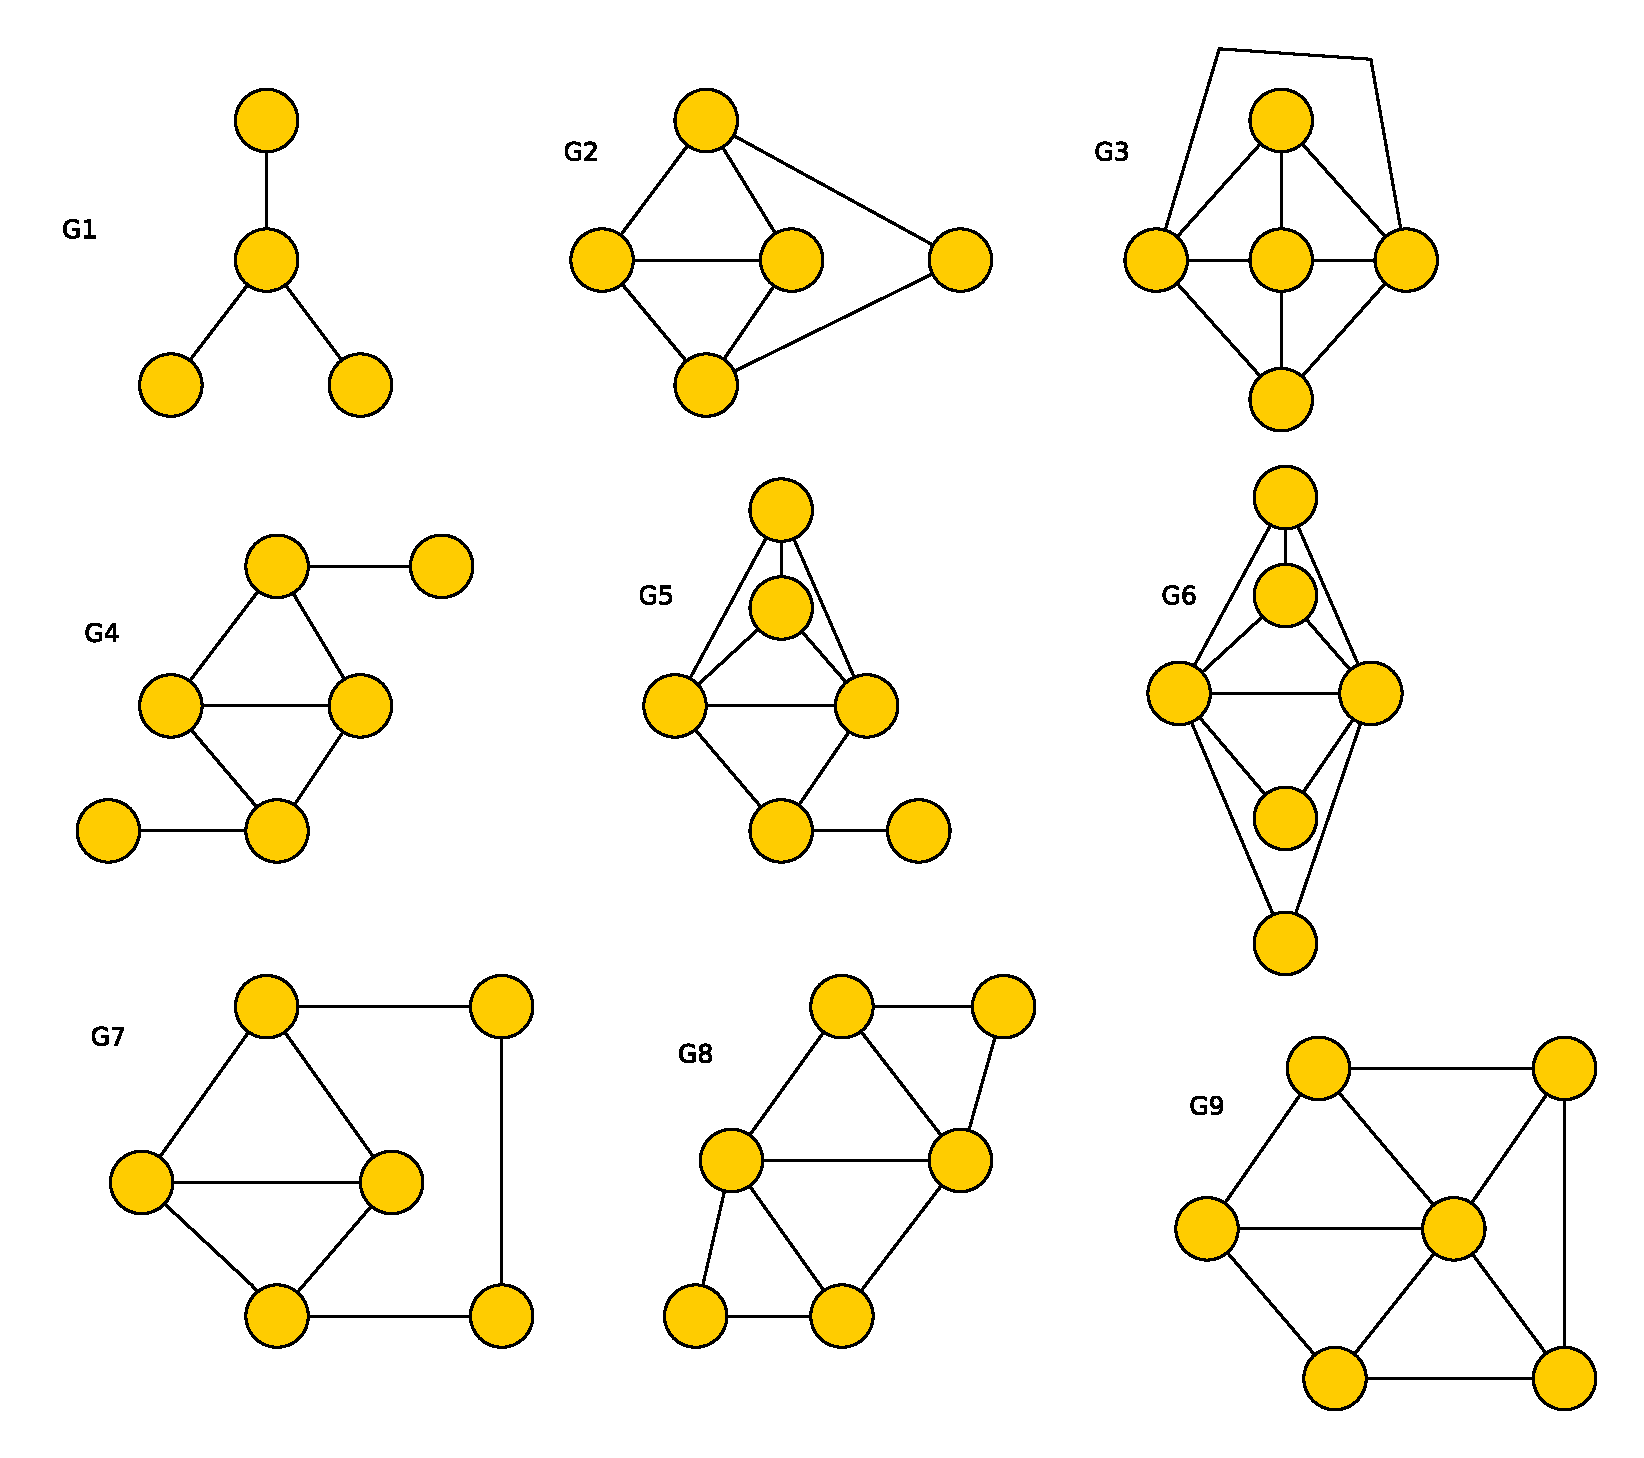
\includegraphics[scale=0.50]{neufSousGraphesInterditDesLineGraphes.eps}\vspace{-0.5em}
	\caption{ Les $9$ sous-graphes interdits dans un line-graphe. }\vspace{-0.5em}
	\label{neufSousGraphesInterditDesLineGraphes}
\end{figure}
% ------ figure neuf Sous Graphes Interdit Des LineGraphes
\FloatBarrier

{\bf Conclusion} :
soit $H$ un graphe et $G$ un graphe non-orient\'e.
Le graphe $H$ est un line-graphe de $G$ si le th\'eor\`eme \ref{caracteristiquesLinegraphes} est respect\'e.
Les graphes $H$ et $L(G)$ sont isomorphes et le graphe racine de $H$ est $L^{-1}(H)$.
Si $H$ est un line-graphe d'un graphe non orient\'e $G$,
alors le graphe $H$ admet un partitionnement en cliques et chaque clique correspond \`a un sommet de $G$. L'ensemble de cliques est appel\'e une {\em couverture de corr\'elation} et est not\'e ${\cal CC}(G)$.

	%------- proprietes_linegraphes -------------------------
	\subsection{Line-graphes ambigus}
		Soient $G$ un graphe non orient\'e et $H$ l'unique  line-graphe de $G$.
D'apr\`es le th\'eor\`eme \ref{caracteristiquesLinegraphes}(b), les ar\^etes de $H$ se partitionnent en cliques telles que chaque clique correspond \`a un sommet de $G$. 
\newline
Si le graphe de correction $G_c$ est sans erreur, alors il est un line-graphe et son partitionnement en cliques forme une {\em couverture de corr\'elation} not\'ee ${\cal CC}(G_c)$.
Existe-t-il plusieurs {\em couvertures de corr\'elation} de $G_c$ c'est-\`a-dire $G_c$ a-t-il plusieurs graphes racines qui sont isomorphes ?
Pour r\'epondre \`a cette question, nous d\'efinissons la notion d'{\em ambigu\"{i}t\'e}. 
\newline

\begin{definition}
Soient $G$ un graphe non orient\'e et $L(G)$ le line-graphe de $G$. 
\newline
Une ambigu\"{i}t\'e dans $L(G)$ est un sous-graphe isomorphe \`a l'un des graphes de la figure \ref{configurationAmbiguite}. Le sommet $X$ est appel\'e le {\bf point d'ambigu\"{i}t\'e}.
\end{definition}

Il a \'et\'e montr\'e que deux line-graphes isomorphes ont leurs graphes racine isomorphes \`a l'exception du graphe triangle \cite{whitney1932congruent}. Les graphes de la figure \ref{configurationAmbiguite} sont isomorphes mais leurs graphes racines ne sont pas isomorphes. Cela implique que leurs couvertures de corr\'elation sont diff\'erentes. D'o\`u la pr\'esence de sommets {\em ambigus}.

\begin{lemma}
	Soient $G = (V,E)$ un line-graphe  et $u$ un sommet de $G$. 
	\newline
	Si $G$ admet deux couvertures de corr\'elation, alors il existe au moins un sommet $u$ de $G$ tel que $G[\{u\} \cup \Gamma_{G}(u)]$ est une ambigu\"{i}t\'e dans laquelle $u$ est le point ambigu\"{i}t\'e.
\end{lemma}
	
\begin{Proof} 
{\em
	Consid\'erons deux couvertures de corr\'elation ${\cal CC}(G)$ et ${\cal CC'}(G)$ de $G$. 
	Il existe au moins un sommet $v \in V[G]$ qui n'est pas couvert par la (ou les) m\^eme(s) clique(s) dans  ${\cal CC}(G)$ et ${\cal CC'}(G)$.
	Soient deux cliques $c_1$ et $c_2$ (potentiellement vide) partitionnant $\{v\} \cup \Gamma_{G}(v)$ dans ${\cal CC}(G)$.
	Consid\'erons deux autres cliques $c_3$ et $c_4$ diff\'erentes de $c_1$ et $c_2$ partitionnant \'egalement $\{v\} \cup \Gamma_{G}(v)$ dans ${\cal CC}(G)$. 
	\newline
	Notons $c_{i,j}$ l'intersection de $c_{i}$ et $c_j$ pour tout $i \in \{1,2\}$ et $j \in \{3,4\}$. 
	Chaque sommet $w \in c_{i,j}$ est couvert par au plus deux cliques de $G$ dans ${\cal CC}(G)$, dont la clique $c_i$.
	Puisque $c_j$ est une clique alors ce sommet $w$ est voisin de tous les sommets de  $c_{i',j}$, pour $i' \ne i$.
	Les ar\^etes entre ces sommets sont dans $c'_i$, donc chaque ar\^ete $[w,z]$ pour tout sommet  $z \in c_{i',j}$ forme une clique dans le r\'eseau de flots.
	Ainsi, le cardinal de chaque ensemble  $c_{i,j}$ est \'egal \`a $1$.\newline
	Appelons $v_{i,j}$ le seul sommet pr\'esent dans $c_{i,j}$. 
	Il est possible d'avoir $v_{1,3} = v_{1,4}$ ou $v_{2,3} = v_{2,4}$.
	Si les deux \'egalit\'es sont v\'erifi\'ees, le sommet $v$ est alors couvert non pas par deux cliques mais par une seule de cardinalit\'e $3$.
	Ainsi, les seuls cas possibles sont alors r\'esum\'es par la figure  \ref{graphe2Couverture}.
	Le sommet $v$ est bien le point d'une ambigu\"{i}t\'e isomorphe \`a $G[\{u\} \cup \Gamma_{G}(u)]$.
} 
\hspace{16 em}$\qed$
\end{Proof}

Nous d\'eduisons le corollaire suivant :
\begin{corollary}
\label{corollaireGraphe2couverture}
Soit $G$ un line-graphe. 
\newline
Si $G$ admet deux couvertures de corr\'elation diff\'erentes, alors il est isomorphe \`a l'un des graphes de la figure  \ref{graphe2Couverture}.
\end{corollary}

% ----- figure configurationAmbiguite
\begin{figure}[htb!]\vspace{-0.5em}
	\centering
	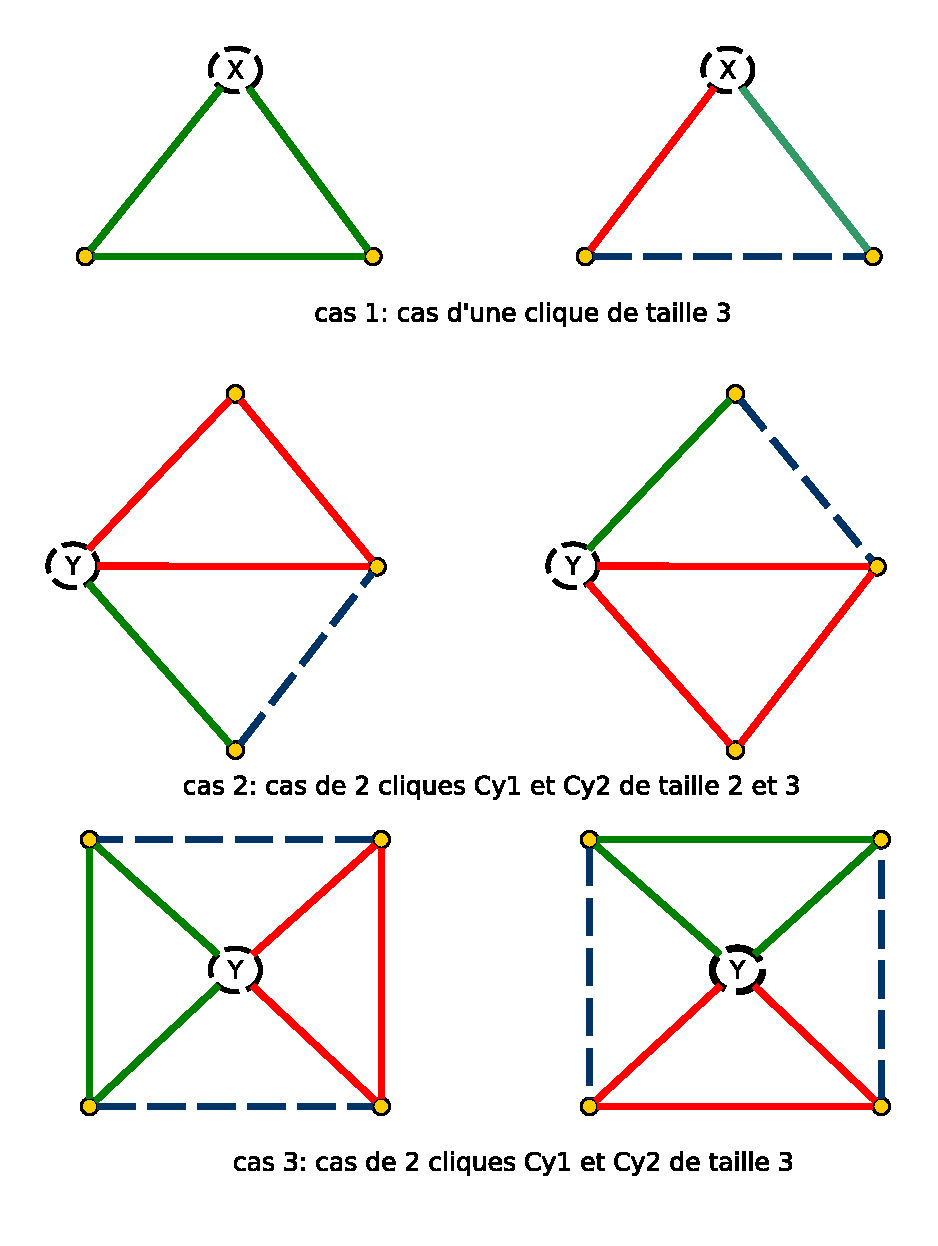
\includegraphics[scale=0.70]{configurationAmbiguite.eps}\vspace{-0.5em}
	\caption{ Configurations possibles d'une ambigu\"{i}t\'e au sommet X. }\vspace{-0.5em}
	\label{configurationAmbiguite}
\end{figure}
% ----- figure configurationAmbiguite
\FloatBarrier


En effet, si $G[\{u\} \cup \Gamma_{G}(u)]$ a une ambigu\"{i}t\'e, chaque ar\^ete, qui n'est pas li\'ee au point d'ambigu\"{i}t\'e, doit \^etre une ar\^ete d'une et une seule autre ambigu\"{i}t\'e de $G$. Et chaque sommet d'une ambigu\"{i}t\'e, qui n'est pas un point d'ambigu\"{i}t\'e, doit appartenir \`a une et une seule autre ambigu\"{i}t\'e de $G$ dont il n'est pas non  plus le point d'ambigu\"{i}t\'e.
De plus, chaque ar\^ete, n'\'etant pas couverte par les deux configurations de cliques possibles dans une ambigu\"{i}t\'e (les ar\^etes en pointill\'ees dans la figure \ref{configurationAmbiguite}), doit \^etre dans une autre ambigu\"{i}t\'e \`a laquelle elle appartient.
Ces contraintes font que si un graphe contient une ambigu\"{i}t\'e induite, alors il ne peut \^etre que dans un cas de la figure  \ref{graphe2Couverture}.

\begin{definition}
\label{cliquesCoherentes}
Soient $G$ un graphe, $u$ un sommet de $G$ et $\Gamma_G(u)$ les sommets voisins de $u$. 
\newline
Une partition de $\Gamma_G(u)$ en deux cliques $C_{u1}, C_{u2}$ est {\bf coh\'erente } si et seulement si chaque sommet $v$ de $C_{u1}$ (resp. $C_{u2}$) a au plus un voisin dans $C_{u2}$  (resp. $C_{u1}$).
\end{definition}

% ---- figure graphe de couverture
\begin{figure}[htb!] \vspace{-1.5em}
\centering
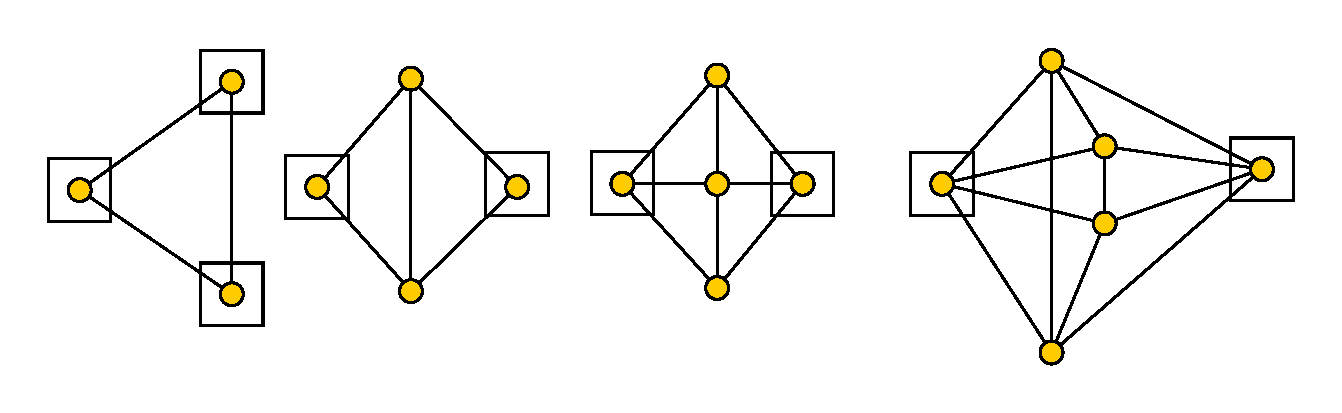
\includegraphics[scale=0.75]{graphe2Couverture.eps}
\caption{ Les graphes possibles de deux couvertures de corr\'elation avec les points d'ambigu\"{i}t\'es encadr\'es. }
\label{graphe2Couverture} 
\end{figure}
% ---- figure graphe de couverture
\FloatBarrier


{\bf Conclusion} : 
nous avons montr\'e que la {\em couverture de corr\'elation} d'un line-graphe est unique \`a l'exception des situations ambigu\"{i}t\'es. Les cas d'ambigu\"{i}t\'es sont pr\'esent\'es dans la figure \ref{graphe2Couverture}.





\section{Formulation du Probl\`eme {\em Proxi-Line}}

	%------- introduction_matrice_correlation ---------
	Soient $G$ un graphe non orient\'e d'un DAG,
 $G_c$ un graphe de corr\'elation de $G$ et 
 $M$ la matrice d'adjacence de $G_c$.
 \newline
 Notre probl\`eme est de d\'eterminer $G$ \`a partir de $G_c$. Pour ce faire, nous d\'ecidons de nous servir de la {\em couverture de corr\'elation}.
On a trois cas :
\begin{itemize}
	\item Soit $G_c$ est isomorphe \`a $L(G)$. Nous trouverons la couverture de corr\'elation unique qui donne $G$.
	\item Soit $G_c$ est un line-graphe non isomorphe \`a $L(G)$. 
		Modifier la matrice d'un line-graphe peut en effet le transformer en un autre line-graphe. Ce cas arrive rarement notamment lorsqu'il y a peu d'ar\^etes erron\'ees dans $G_c$. 
	\item Soit $G_c$ n'est pas un line-graphe. Dans ce cas, l'id\'ee est de corriger $G_c$ en ajoutant ou supprimant le minimum d'ar\^etes.
\end{itemize}
Nous resolvons le $3^{ieme}$ cas en introduisant le probl\`eme suivant :



	%------- probleme -----------------------------------------------
	\subsection{Probl\`eme}
		\'Etant donn\'e un graphe $G'$ qui a des ar\^etes en plus ou en moins par rapport \`a un autre graphe $G$ de m\^eme ensemble de sommets.
\begin{definition}
%La distance en $G$ et $G'$ est la distance de Hamming not\'ee $DH(G,G')$ entre leurs deux matrices d'adjacente, c'est-\`a-dire le nombre d'\'el\'ements ayant une valeur diff\'erente dans chacune des deux matrices.
Soient $G$ et $G'$ deux  graphes non orient\'es ayant le m\^eme ensemble de sommets.
\newline
La distance de Hamming entre les graphes $G$ et $G'$ not\'ee $DH(G,G')$ est le nombre d'ar\^etes pr\'esentes dans $G$ et pas $G'$ et inversement.
\end{definition}
Une distance de Hamming \'egale \`a $k$ $(k \in \mathbb{N})$ signifie qu'il existe $k$ cases diff\'erentes entre les matrices d'adjacence des graphes $G$ et $G'$.


\begin{definition}
Soit $G$ un graphe non orient\'e.
\newline
On appelle {\em distance line} de $G$, not\'ee $DL(G)$, la plus petite distance de Hamming entre $G$ et $G'$, un line-graphe ayant le m\^eme ensemble de sommets que $G$.
\end{definition}


Nous consid\'erons le probl\`eme suivant. \newline
{\bf Probl\`eme} Proxi-Line \newline
{\bf Donn\'ees} : Un graphe $G=(V,E)$, un entier $k$. \newline
{\bf Question} : $DL(G) \le k$ ? 
\newline


\begin{conjecture}
Proxi-Line est NP-complet.
\end{conjecture}

Ce probl\`eme g\'en\'eralise le probl\`eme {\em NP-complet} d\'efini et montr\'e  dans \cite{yannakakis1978node}, c'est-\`a-dire \'etant donn\'es un graphe $ G $ et un entier $k$, le probl\`eme de savoir s'il existe un line-graphe $ G'$ qui est un sous-graphe couvrant de $ G $ tel que $ dH (G, G' ) \leq k $ (c'est-\`a-dire, le probl\`eme Proxi-Line dans lequel seule la suppression d'ar\^etes  est autoris\'ee) utilise une solution de programmation lin\'eaire en nombres entiers   dans \cite{Halldorsson2013}. R\'ecemment, il a \'et\'e montr\'e au sein du laboratoire DAVID que l'op\'eration d'ajout d'ar\^etes uniquement dans le graphe de corr\'elation est aussi  {\em NP-complet}.


	%------- Conclusion description algorithmes -----------------------------------------------
%	\subsection{Conclusion de la formulation du probl\`eme}
%		
Nous avons consid\'er\'e que
la couverture de corr\'elation du graphe de corr\'elation $G_c$ est unique m\^eme en pr\'esence d'erreurs de corr\'elations et d'ambigu\"{i}t\'es.  La d\'etermination du graphe $G$ non orient\'e sous-jacent au DAG est ais\'ee.
\newline
Dans le cas o\`u la d\'etermination de couverture de corr\'elation de $G_c$ est impossible, nous avons d\'efini le probl\`eme {\em Proxi-Line}. Le but de {\em Proxi-Line} est de fournir le line-graphe de $G$ qui a le minimum d'ar\^etes diff\'erent par rapport $G_c$.  

%-----------------------------------------------------------------------------------------------------------
%------- algorithme de decouverte: couverture et correction ---------------------
%-----------------------------------------------------------------------------------------------------------
\section{Algorithmes de d\'ecouverte de topologie}

	
%%%%% ---- commentaire dominique pour l'intro
%Dire ce que cest le probleme tu regarde
%qu'est ce qui existe pour resoudre proxiline
%etant donn\'ee u graphe pour reconnaitre que cest un line graphe ou pas
%%%%% ---- commentaire dominique pour l'intro

Le probl\`eme consid\'er\'e ici est, 
\'etant donn\'e un graphe, de d\'eterminer s'il est un line-graphe et dans ce cas donner le graphe racine.
Nous d\'ebutons par l'\'etat de l'art des algorithmes de couverture en cliques puis pr\'esentons nos algorithmes tout en sp\'ecifiant leurs particularit\'es par rapport aux m\'ethodes existantes. 

\subsection{Recherche de Couverture en cliques}
Diff\'erents travaux ont \'et\'e r\'ealis\'es sur la d\'ecouverte de {\em couverture en cliques} dans les line-graphes.
Parmi lesquelles, nous citons  l'algorithme de {\em Roussopoulos}  \cite{ROUSSOPOULOS1973108} qui utilise une propri\'et\'e des line-graphes provenant des travaux de {\em Krausz} \cite{krausz1943demonstration}. 
Il affirme que le graphe $G$ est un line-graphe si ses ar\^etes  peuvent \^etre partitionn\'ees en cliques  de telle sorte qu'aucun sommet ne soit couvert par plus de deux cliques. 
L'algorithme propos\'e d\'etecte si $G$ est un line-graphe et il fournit, en plus, son graphe racine en temps lin\'eaire $O(max(\{m,n\}))$, avec $n$ et $m$ les nombres respectifs de sommets et d'ar\^etes.
\newline
Un autre algorithme, propos\'e par {\em Klauss Simon} et {\em Daniele Degiorgi} \cite{decompositionEnCliques}, est une simplication du probl\`eme de reconnaissance de line-graphes. Bas\'e sur la preuve de {\em Oystein Ore} du th\'eor\`eme de {\em Whitney} \cite{whitney1932congruent}, il stipule que deux line-graphes connexes avec plus de quatre sommets sont isomorphes si et seulement si leurs graphes racines sont aussi isomorphes et que ces graphes  doivent \^etre diff\'erents de $K_{1,3}$ et $K_3$. Il d\'etermine en un temps lin\'eaire une couverture \'etant mise \`a jour sommet apr\`es sommet. 
L'inconv\'enient de cette m\'ethode est le traitement de sommets appartenant \`a des cliques ayant d\'ej\`a \'et\'e d\'ecouverts parce qu'il applique le partitionnement sur la liste des sommets obtenus.
\newline
L'algorithme de {\em Philippe Lehot} \cite{decompositionEnCliquesParArcs} a une complexit\'e en $O(n) + m$ avec $n$ le nombre de sommets de $G$ et $m$ le nombre d'ar\^etes de $L(G)$.
Il recherche les $9$ sous-graphes de la figure \ref{neufSousGraphesInterditDesLineGraphes} et il utilise le th\'eor\`eme de {\em Van Rooij et Wilf} \cite{ROOIJetWILF1965interchange} qui \'enonce qu'un graphe $G$ est un line-graphe si $G$ ne contient pas de sous-graphe induit $K_{1,3}$ et si deux graphes triangles  {\em impairs} ont une ar\^ete commune, alors le sous-graphe induit par ces sommets est une clique $K_4$. 
Rappelons qu'un graphe triangle (c'est-\`a-dire un cycle de longueur $3$) $\{a_1,a_2,a_3\} \subseteq V(L(G))$ est {\em impair} s'il existe un sommet $e \in V(G)$ adjacent \`a  au moins un des sommets $\{a_1, a_2, a_3\}$. Ce triangle est {\em pair} si chaque sommet de ce triangle est adjacent \`a $0$ ou $2$ autres sommets. Cet algorithme est d\'etaill\'e dans la section \ref{algoCouverture}.
%% graphe odd = impair/ even=pair
%A triangle in a graph is even if every other node is adjacent to 0 or 2 nodes in the triangle; it is odd otherwise. 
%%
\newline
Tous les algorithmes existants ne retournent  aucun r\'esultat lorsque le graphe  de corr\'elation $G_c$ poss\`ede des cases erron\'ees c'est-\`a-dire qu'il n'est pas un line-graphe. 
Cependant, la m\'ethode propos\'ee par {\em Halld{\'o}rsson and al.} \cite{Halldorsson2013} 
utilise un algorithme g\'en\'etique pour corriger un graphe de corr\'elation pour en obtenir un line-graphe. 
En effet, il propose une m\'ethode de d\'ecouverte de la g\'en\'ealogie de population en se basant sur les haplotypes partag\'es dans les g\'enomes des individus.  
Un haplotype est un groupe d'all\`eles dans un organisme qui est transmis ensemble par un parent.
Il mod\'elise un graphe dit {\em Clark Consistency} \cite{halldorsson2011clark} dans lequel les ar\^etes sont les haplotypes (ils sont uniques dans les g\'enomes) et les sommets sont les individus.
Cette m\'ethode recherche le graphe racine induit par le graphe {\em Clark Consistency} si celui ci est un line-graphe. Dans le cas o\`u le graphe {\em Clark Consistency graph} n'est pas un line-graphe, l'algorithme suppose qu'il existe des sommets en plus dans le {\em graphe Clark Consistency}, va les supprimer afin que le graphe devienne un line-graphe et enfin retourner le graphe racine.     
Le graphe {\em Clark consistency (CC)} a \'et\'e propos\'e dans  la m\'ethode d'identification d'haplotypes par {\em Andrew Clark}. 
En effet, {\em Andrew Clark} consid\`ere un ensemble de g\'enomes d'individus qui ont des haplotypes homozygotes et h\'et\'erozygotes. Il suppose que deux g\'enomes n'ont pas les m\^emes paires d'haplotypes. Les sommets du graphe CC sont les g\'enomes des individus et une ar\^ete de graphe CC entre deux g\'enomes existe s'ils partagent le m\^eme haplotype (homozygote ou h\'et\'erozygote). Les ar\^etes de ce graphe sont form\'ees par des individus partageant les m\^emes haplotypes. 
%%%
%A key component of our approach is the graph of potential sharing of haplotypes between individuals. This graph, called the Clark consistency (CC) graph, was first suggested in the context of a method for haplotype phasing by Andrew Clark [10]. Given the genotypes of a set of individuals, the CC graph has one node for each individual and an edge between two individuals if their genotypes are consistent with sharing a haplotype, i.e., if for every site where one of the individuals is homozygous, the other individual is either homozygous for the same allele or heterozygous. As the haplotypes of individuals that are homozygous for the whole region being considered are easily determined, we assume that every given individual has two different haplotypes (i.e., it is heterozygous for at least one of the genotyped markers) and no two individuals have the same pair of haplotypes.
%%%
Le probl\`eme de d\'ecouverte de line-graphes \'etant {\em NP-Complet}, la solution propos\'ee r\'ealise un algorithme de suppression de sommets et d'ar\^etes. 
L'algorithme de suppression de sommets est une 6-approximation alors que celui des ar\^etes est de complexit\'e $O(n*m)$ avec $m$ le nombre de sommets et $n$ le nombre d'ar\^etes.
Dans le cas o\`u des suppressions sont effectu\'ees, le line-graphe fourni est le plus proche possible du line-graphe de l'arbre g\'en\'ealogique.
La particularit\'e de la solution est l'absence d'ar\^etes ajout\'ees dans le line-graphe et cela implique que cette solution est inapplicable dans notre probl\`eme o\`u il existe des ar\^etes inconnues dans notre graphe de corr\'elation. En plus, l'ensemble de nos sommets dans le graphe de corr\'elation est connu contrairement \`a l'algorithme de {\em Halld{\'o}rsson et al.} qui suppose que les sommets doivent \^etre supprim\'es pour atteindre un line-graphe.
\newline
Nous nous basons sur l'algorithme de {\em Lehot} parce qu'il s'ex\'ecute en un temps lin\'eaire en effectuant un traitement sommet par sommet pour la reconnaissance de sous-graphes complets. Ce traitement permet de s\'electionner les cliques existantes et les sommets, n'appartenant \`a aucune clique, qui n\'ecessitent une modification de leur voisinage.
	
	%------- algo couverture -----------------------------------------------
	\subsection{Algorithme de couverture}
		\label{algoCouverture}
		% description de l'algo de lehot
L'algorithme de {\em couverture} que nous proposons est une am\'elioration de celui de {\em Lehot}.
Ainsi, nous pr\'esentons tout d'abord bri\`evement le principe de l'algorithme de couverture en cliques de {\em Lehot} \cite{decompositionEnCliquesParArcs}. 
\newline
Soient $H$ et $G$ deux graphes. Nous supposons que $H$ est le line-graphe de $G$ ($H=L(G)$).
Le but de cet algorithme est d'identifier le graphe racine $L^{-1}(H)$ de $H$.
L'algorithme va construire $G$  au fur et \`a mesure en identifiant les cliques dans $H$. 
Les ar\^etes et les sommets de $H$ et $G$ peuvent avoir au cours de l'ex\'ecution plusieurs \'etats :
%''----------- sommets de H et G 
\begin{itemize}
	\item Sommet ``bien-d\'efini'' : un sommet d\'ecouvert de $G$ tel que la clique correspondante dans $H$ a \'et\'e trouv\'ee et identifi\'ee.
	\item Sommet ``\`a moiti\'e-nomm\'e'' :  un sommet de $H$ tel que  l'ar\^ete correspondante dans $G$ a une extr\'emit\'e  ``bien-d\'efinie''. 
	\item Sommet ``pleinement-nomm\'e'' : un sommet de $H$ tel que l'ar\^ete correspondante dans $G$  a des extr\'emit\'es ``bien-d\'efinies''.
	\item Sommet ``basique'' : un sommet de $H$ est une ar\^ete de $G$. Ces sommets sont not\'es $x-y$ dans $H$ avec $x$ et $y$ des sommets d\'ecouverts de $G$.
	\item Sommet ``partag\'e'' : sommet de $H$ partageant une ar\^ete avec des sommets ``basiques'' adjacents. Ce sommet est une extr\'emit\'e commune entre des ar\^etes de $G$ incidentes. 
\end{itemize}
%''----------- sommets de H et G 


L'id\'ee de cet algorithme est de d\'eterminer une couverture de corr\'elation de $H$ en d\'etectant, selon $3$ cas \cite{decompositionEnCliquesParArcs} dans $H$, 
les sommets partag\'es adjacents \`a un sommet ``basique'' qui forment une clique.
Nous illustrons le fonctionnement de l'algorithme avec l'exemple suivant illustr\'e par la figure \ref{deroulementAlgorithmeLehotRechercheSommetsPartages}.
L'algorithme s\'electionne deux sommets ``basiques''  $1-2, 2-3$ et  l'ensemble $X$ des sommets adjacents aux sommets ``basiques''.
Si $X = \emptyset$ alors il n'existe pas de sommet partag\'e dans  $G$ et les sommets $1-2, 2-3$ sont \'etiquet\'es ``\`a moiti\'e nomm\'e'' (figure \ref{deroulementAlgorithmeLehotRechercheSommetsPartages}(a)).
Si $X=\{x\}$ alors le sommet $x$ est un sommet partag\'e dans  $H$ si $x = 2-4$ car le triangle $\{x, 1-2, 2-3\}$ est impair. Dans le cas o\`u $x = 1-3$, le  triangle $\{x, 1-2, 2-3\}$ est pair et
aucun sommet d\'ecouvert dans $G$ n'est incident aux sommets du triangle $\{x, 1-2, 2-3\}$ (figure \ref{deroulementAlgorithmeLehotRechercheSommetsPartages}(b)). 
Le sommet $x$ dans $H$ est \'etiquet\'e ``pleinement-nomm\'e'' et les autres sommets $1-2, 2-3$ dans $H$ sont \'etiquet\'es ``\`a moiti\'e nomm\'es''.
Si $X=\{x,y\}$, il n'existe  aucun sommet partag\'e dans  $H$ si $x$ et $y$ sont adjacents dans $H$. Dans le cas o\`u  ils ne sont pas adjacents alors ils forment deux triangles avec $1-2, 2-3$. Si $x=2-4$ et $y=1-3$ alors le triangle $\{2-4,1-2, 2-3\}$ est impair et $x$ est le sommet partag\'e dans $H$
(figure \ref{deroulementAlgorithmeLehotRechercheSommetsPartages}(c)).
Enfin pour $|X| = |\{a,b,c, \cdots\}| = 3$, le sommet $b$ dans $H$ est \'etiquet\'e sommet partag\'e si $a$ est adjacent \`a $b$ sinon le sommet $a$ devient le sommet partag\'e.
La derni\`ere \'etape s\'electionne al\'eatoirement un sommet ``\`a moiti\'e-nomm\'e'' dans $H$ qui est adjacent \`a un sommet  ``pleinement-nomm\'e'' dans $H$. Si ce sommet n'est pas d\'ej\`a couvert par une clique alors il est ``pleinement-nomm\'e'' et il est un sommet partag\'e dans $H$. 
\`A la fin de cette \'etape, tous les sommets sont \'etiquet\'es \`a ``pleinement-nomm\'e"  dans $H$ et ils deviennent des sommets partag\'es dans $H$.
\newline
L'algorithme s'ex\'ecute  en $O(m)+m'$ avec $m$  le nombre d'ar\^etes dans $G$ et $m'$ le nombre d'ar\^etes dans $L(G)$. Il retourne la liste de cliques d\'ecouvertes dans $H$ dans laquelle chaque clique correspond  \`a un sommet de $G$. Cette liste de cliques est appel\'ee {\em couverture de corr\'elation} (${\cal CC}$).
Malheureusement, si $H$ n'est pas un line-graphe alors il ne retourne pas de couverture partielle.

\subsubsection{Description de l'algorithme de couverture}
Nous proposons  l'algorithme de {\em couverture} (voir algorithme \ref{algo:couverture}) en lien avec celui de {\em Lehot} qui couvre  autant que possible les sommets du graphe de corr\'elation  $G_c$ par une ou deux cliques.
Notre algorithme retourne la {\em couverture de corr\'elation} (${\cal CC}$) de $G_c$ si la matrice d'adjacence de $G_c$ ne contient aucune case erron\'ee sinon il renvoie une {\em couverture de corr\'elation partielle} de $G_c$.
\newline
%% ---- figure etapes de decouverte de l'algo de lehot
\begin{figure}[htb!]
	\centering
	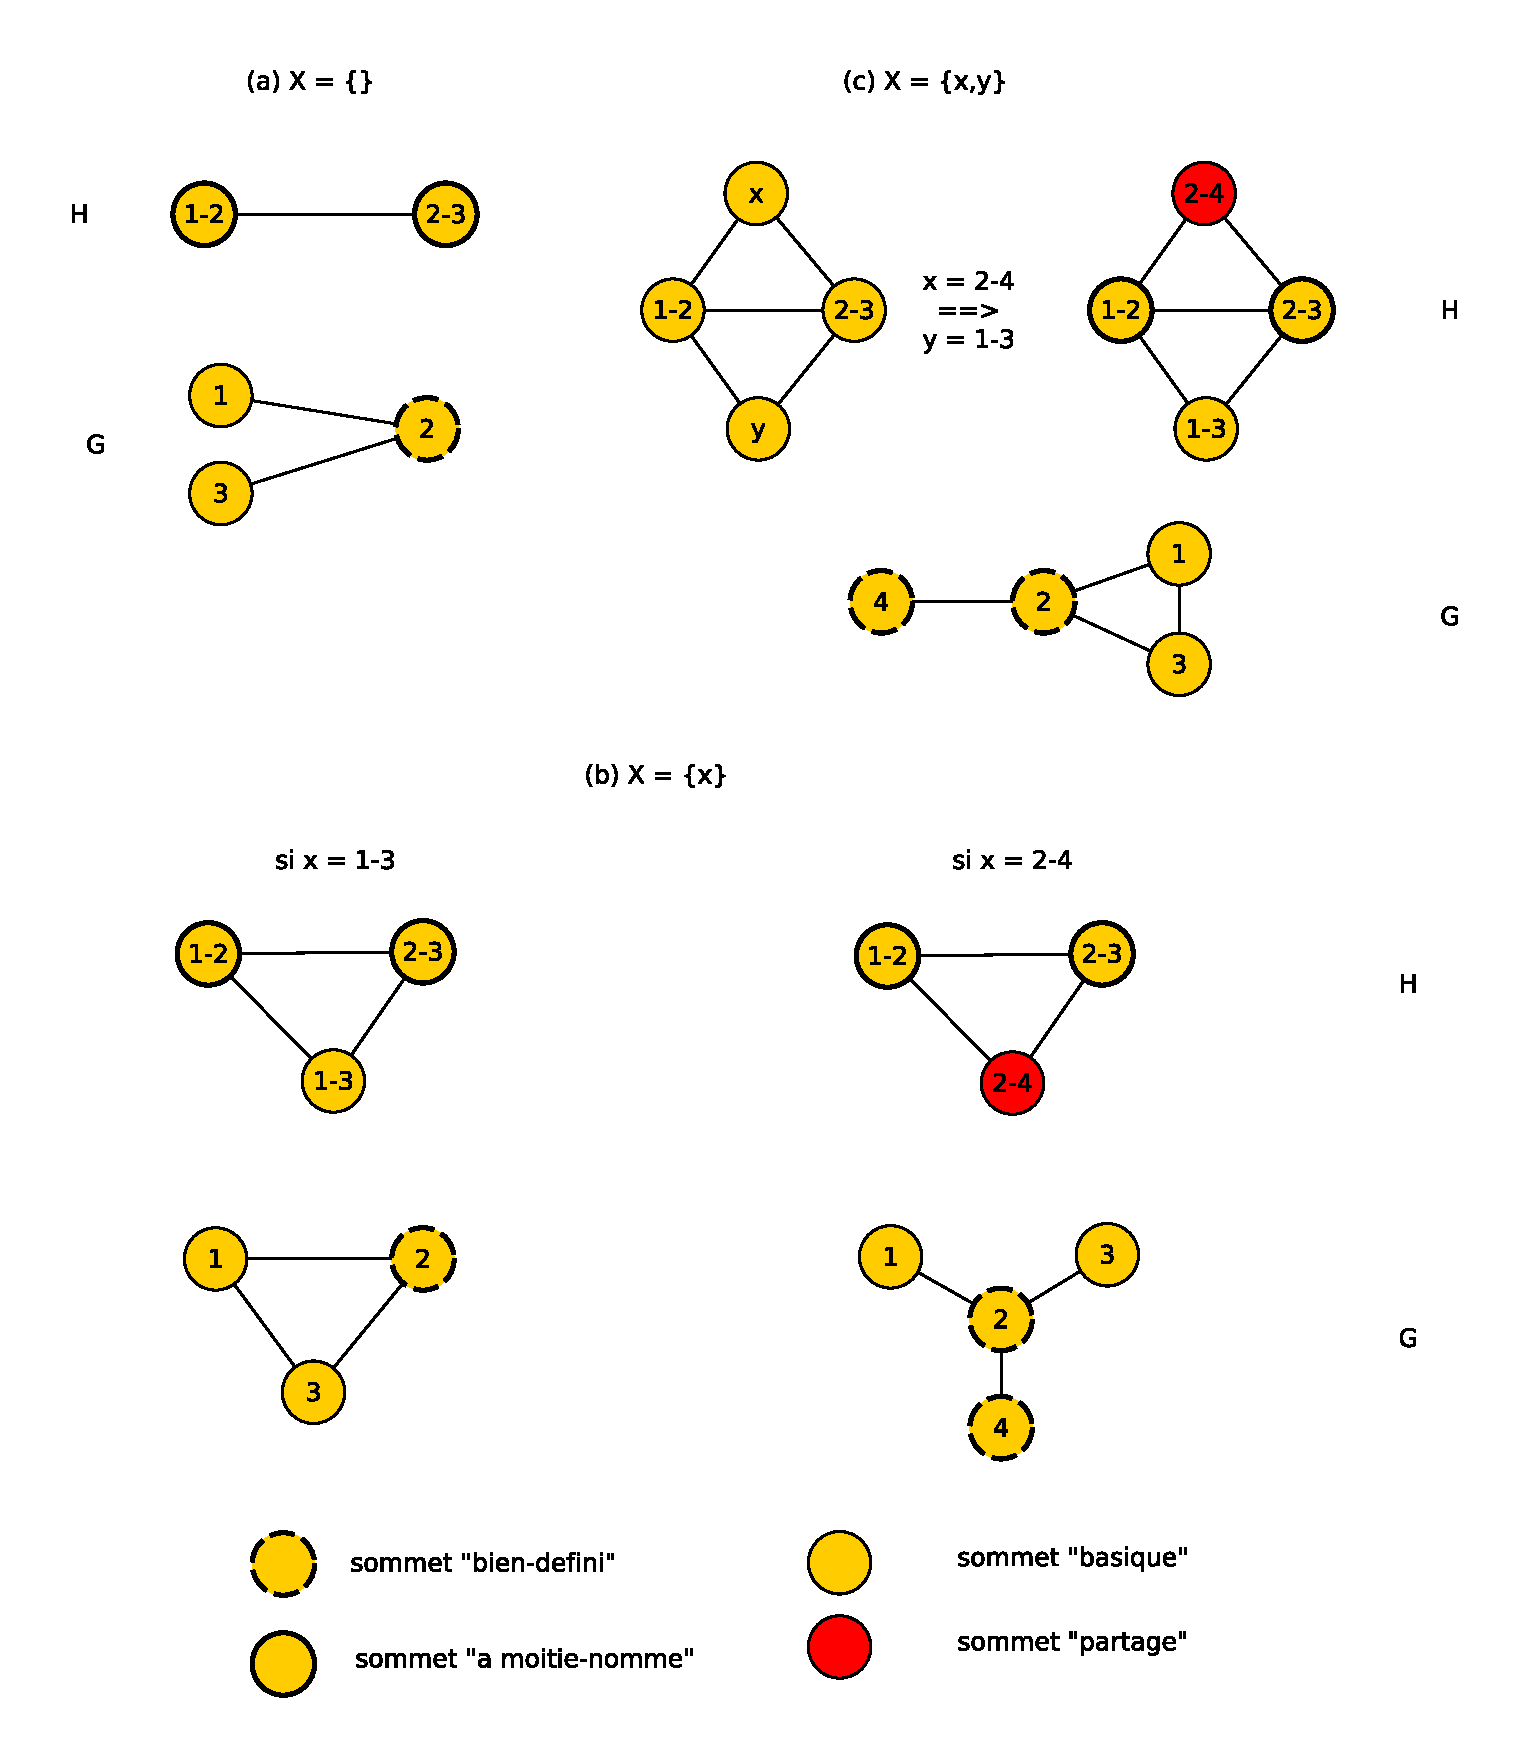
\includegraphics[scale=0.50]{deroulementAlgorithmeLehot.eps}\vspace{-0.5em}
	\caption{ Identification des sommets partag\'es dans le graphe $H$ et nommage des sommets de $G$. }\vspace{-0.5em}
	\label{deroulementAlgorithmeLehotRechercheSommetsPartages}
\end{figure}
%% ---- figure etapes de decouverte de l'algo de lehot
\FloatBarrier

Soient $G_c = (V,E)$ un graphe de corr\'elation et $Cliq(v)$ l'\'etat de chaque sommet $v$ de   $G_c$.
L'algorithme de {\em couverture} va construire une couverture de corr\'elation ${\cal CC}(G_c)$ de $G_c$ en ajoutant des cliques d\'ecouvertes dans ${\cal CC}(G_c)$.  
Une clique est un ensemble de sommets qui induit un sous-graphe complet. 
Si un sommet appartient \`a une clique alors il est couvert par cette clique. 
De m\^eme, si deux sommets $u$ et $v$ appartiennent \`a une m\^eme clique, alors la clique couvre l'ar\^ete $[x,y]$.
Initialement ${\cal CC}(G_c)$ est vide et chaque sommet de $v \in V$ a un \'etat $Cliq(v)=0$. 
\newline
\`A chaque \'etape de l'algorithme, chaque sommet $v$ a $5$ \'etats possibles :
\begin{itemize}
	\item $Cliq(v)=0$ : le sommet $v$ n'est couvert par aucune clique. Il correspond \`a un sommet ``basique'' dans l'algorithme de {\em Lehot}.
	\item $Cliq(v)=1$ : le sommet $v$ est couvert par une clique ou deux cliques. Dans le cas o\`u il est couvert par deux cliques, l'intersection de ces cliques donne le sommet $v$. Ce sommet est \'etiquet\'e ``pleinement-nomm\'e" dans l'algorithme de {\em Lehot}.
	\item $Cliq(v) = 2$ : le sommet $v$ est couvert par une clique et peut \^etre couvert par une seconde clique. Ce sommet est ``bien-nomm\'e" dans l'algorithme de {\em Lehot}.
	\item $Cliq(v) = 3$ : le sommet $v$ est un sommet ambigu. L'algorithme doit identifier la clique \`a laquelle il appartient pour qu'elle devienne un sommet partag\'e dans l'algorithme de {\em Lehot}.
	\item $Cliq(v) = -1$ :  le sommet $v$ est couvert par plus de deux cliques. Il est contenu dans l'ensemble $\cal C$ et doit \^etre corrig\'e par l'algorithme de correction.
\end{itemize}

Nous choisissons un sommet $v$ de degr\'e minimum qui n'appartient \`a aucune clique ou qui est un sommet ambigu. 
S'il existe une partition coh\'erente (voir d\'efinition \ref{cliquesCoherentes}) de ce sommet et de son voisinage $\{v\} \cup \Gamma_{G_c}(v)$ en deux cliques $C_1, C_2$, alors ces deux cliques sont contenues dans la couverture de corr\'elation ${\cal CC}(G_c)$ en cours de construction. Les sommets $v$ et $u$ (avec $u \in  \Gamma_{G_c}(v)$), appartenant \`a $C_1$ ou $C_2$, ont leur \'etat modifi\'e \`a chaque \'etape de l'algorithme de la mani\`ere suivante :
\begin{itemize}
\item $Cliq(v) = 1$ si son \'etat pr\'ec\'edent est \'egal \`a $0$ et la clique $C_2$ est vide. 
\item $Cliq(v) = 3$ si son \'etat pr\'ec\'edent est \'egal \`a $0$ et la clique $C_2$ est non vide. 
\item $Cliq(v) = 2$ si son \'etat pr\'ec\'edent est diff\'erent de $0$.
\item $Cliq(u) = 1$ si son \'etat pr\'ec\'edent est \'egal \`a $0$ et l'ensemble des ar\^etes incidentes \`a $u$ est vide.
\item $Cliq(u) = 2$ si son \'etat pr\'ec\'edent est \'egal \`a $3$ et l'ensemble des ar\^etes incidentes \`a $u$ est vide.
\item $Cliq(u) = 3$ si son \'etat pr\'ec\'edent est \'egal \`a $0$ et l'ensemble des ar\^etes incidentes \`a $u$ est non vide.
\item $Cliq(u) = -1$ si son \'etat pr\'ec\'edent est \'egal \`a $3$ et l'ensemble des ar\^etes incidentes \`a $u$ est non vide.
\end{itemize} 
Dans le cas o\`u il n'existe aucune partition coh\'erente (voir d\'efinition \ref{cliquesCoherentes}) au sommet $v$, son \'etat est \`a $Cliq(v)=-1$.
\newline
%\vspace{-1.5cm}
  %% ---- figure etapes de decouverte de l'algo de lehot
\begin{figure}[htb!]
	\centering
	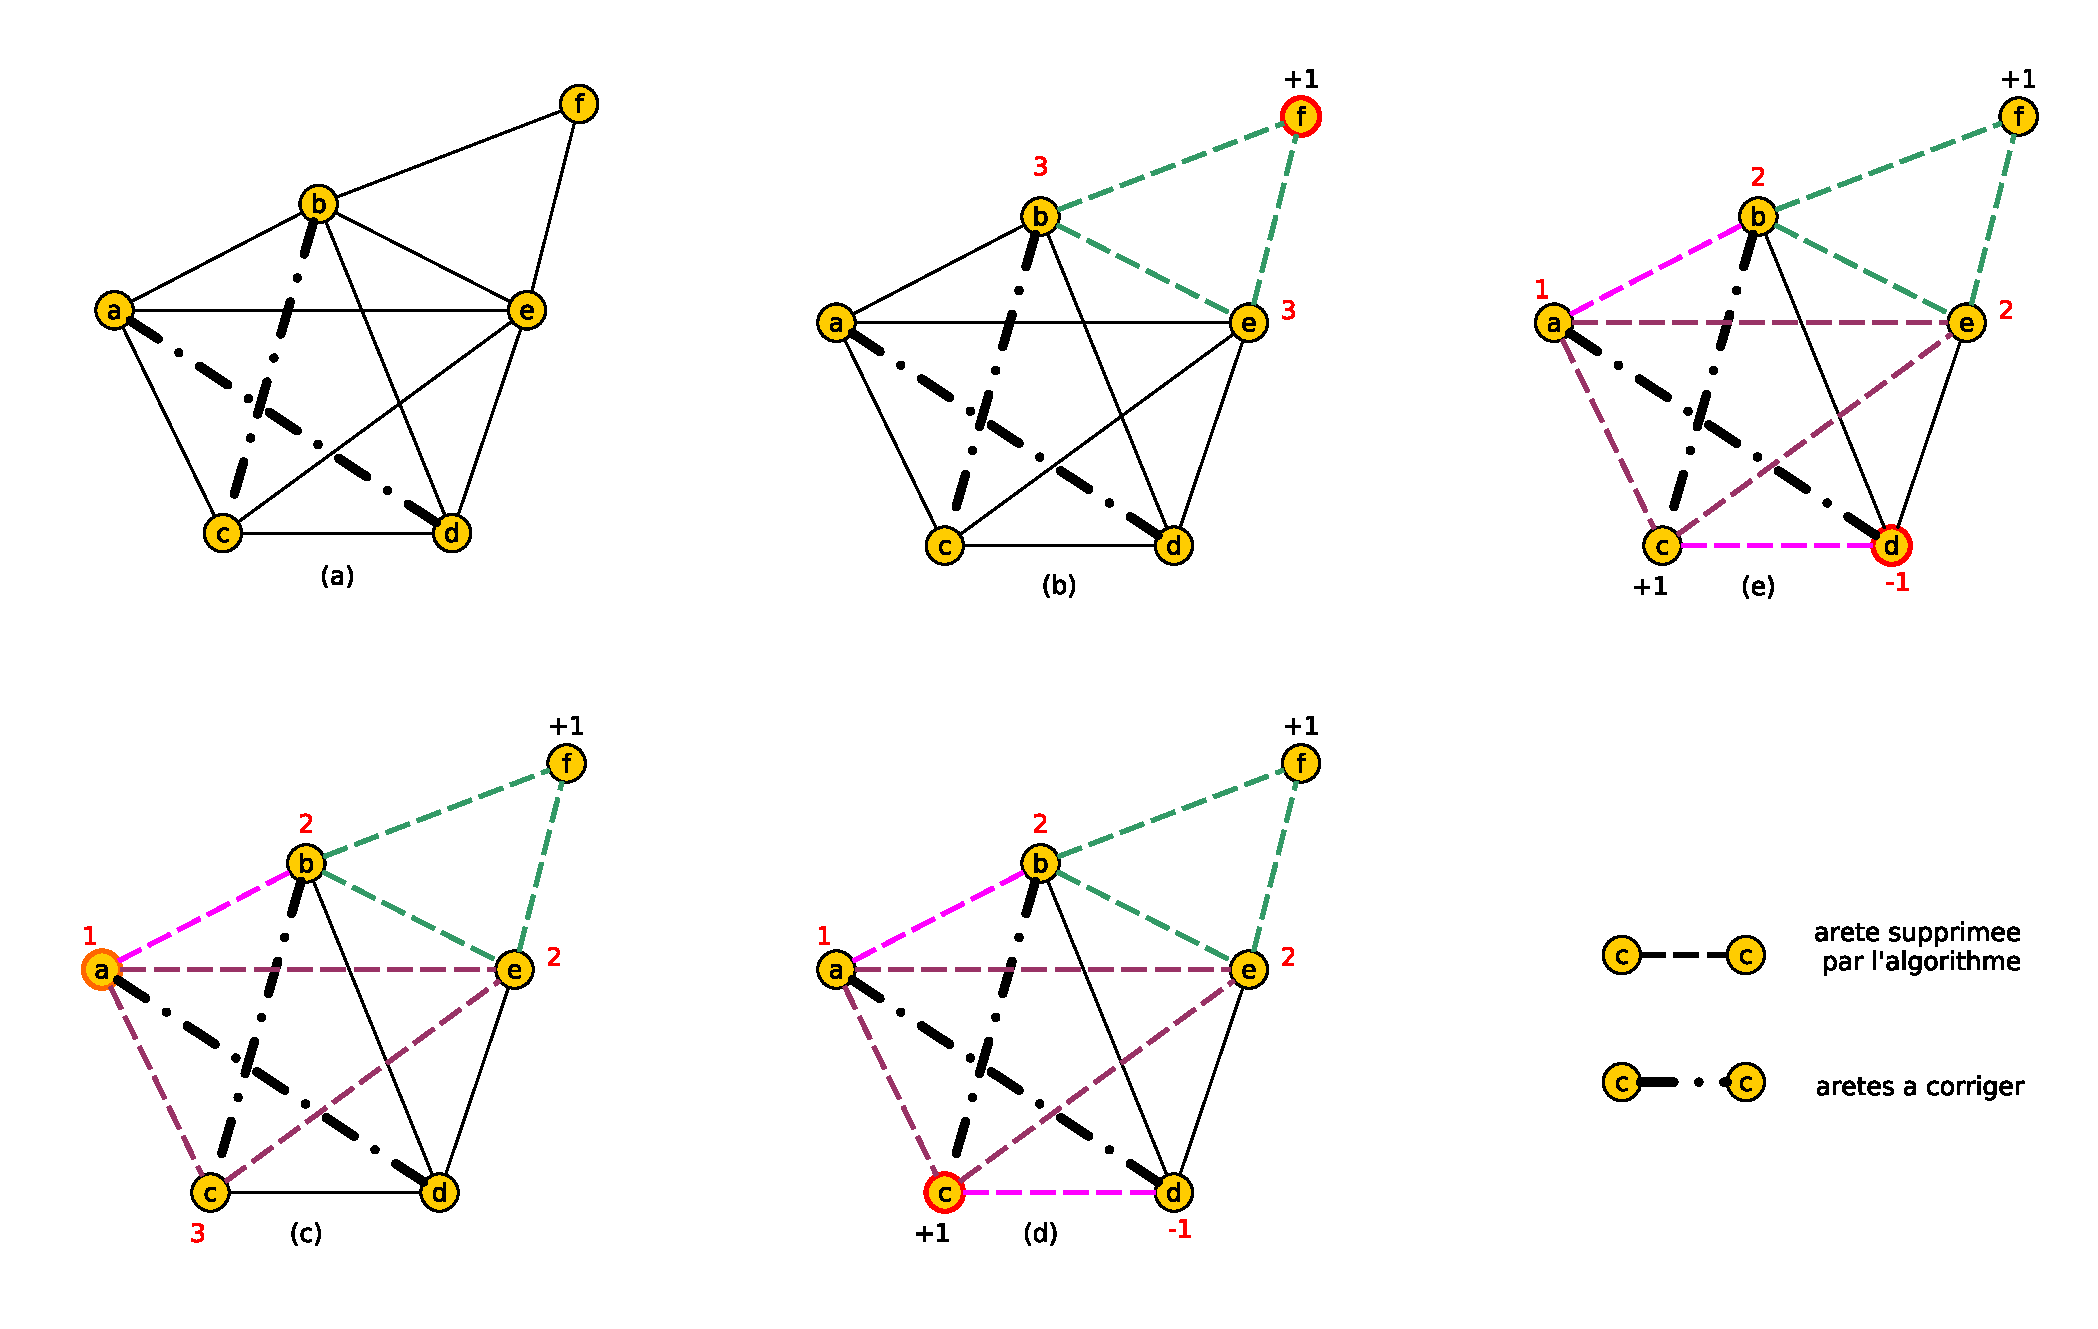
\includegraphics[width=500pt, height= 300pt]{exempleAlgorithmeCouverture.eps}\vspace{-0.5em}
	\caption{ Les diff\'erentes \'etapes de la couverture en cliques du graphe $G$. Les ar\^etes de m\^eme couleur appartiennent \`a la m\^eme clique.  Les ar\^etes $(b,c)$ et $(a,d)$ sont supprim\'ees du graphe avant l'ex\'ecution de l'algorithme de {\em couverture}.  }\vspace{-0.5em}
	\label{exempleAlgorithmeCouverture}
\end{figure}
%% ---- figure etapes de decouverte de l'algo de lehot
\FloatBarrier
%% description de l'algo
L'algorithme de recherche de couverture de corr\'elation ${\cal CC}(G_c)$ (voir algorithme \ref{algo:couverture})  consid\`ere, tant qu'il en existe, un sommet $v$ dont les ar\^etes incidentes sont couvertes par une seule clique. 
Il affecte \`a ce sommet l'\'etat $Cliq(v) = 1$, sauvegarde cette clique dans ${\cal CC}(G_c)$ puis supprime ces ar\^etes incidentes dans le graphe $G_c$. Les voisins de ce sommet passent \`a l'\'etat $2$.
\newline
Si au cours de l'ex\'ecution un tel sommet $v$ n'existe pas alors l'algorithme de {\em couverture} consid\`ere un sommet $u$ dont son voisinage peut \^etre couvert par deux cliques et qui n'a pas \'et\'e pr\'ec\'edemment couvert par une clique de ${\cal CC}(G_c)$. 
Si cette partition en deux cliques est unique, l'algorithme affecte $Cliq(u) = 1$ \`a ce sommet et supprime les ar\^etes. 
Dans le cas o\`u ce sommet appartient \`a un des cas de la figure \ref{configurationAmbiguite} (cas d'un sommet encadr\'e), nous avons montr\'e que ces graphes sont les seuls line-graphes pour lesquels deux partitions possibles existent. 
Nous utilisons la fonction de d\'ecision  $Verif-correl$  (section \ref{VerifCorrel}) pour lever l'ambigu\"{i}t\'e.
\newline
Un \'etat est affect\'e aux autres sommets $v$ de la clique couvrant $v$ selon l'un des trois cas. 
Dans le premier cas, l'\'etat actuel appartient \`a $Cliq(v) \in \{2,3\}$ si les sommets $v$ ont des ar\^etes incidentes non encore couvertes par une clique et l'\'etat pr\'ec\'edent est $Cliq(v) \in \{ 3,0\}$. 
Dans le second cas, $Cliq(v) = 1$ est attribu\'e aux sommets $v$ si l'ensemble des ar\^etes incidentes est vide. 
Enfin, dans le dernier cas, l'algorithme  affecte $Cliq(v) = -1$ \`a ces sommets si leur \'etat pr\'ec\'edent est  $Cliq(v) \in \{2,3\}$ et leurs ar\^etes incidentes ne forment pas une clique.
\newline
\`A la fin  de l'ex\'ecution de cet algorithme, tous les sommets $v$ dont l'\'etat courant est $Cliq(v) = -1$  n'ont pas \'et\'e couverts. 
Ces sommets appartiennent \`a l'ensemble $\cal C$ des sommets \`a corriger par l'algorithme de correction.
\newline

 La figure \ref{exempleAlgorithmeCouverture} d\'etaille l'algorithme de {\em couverture} (algorithme \ref{algo:couverture})  sur un graphe $G=(V,E)$  dans lequel nous avons supprim\'e deux ar\^etes. L'objectif de la suppression d'ar\^etes dans la figure \ref{exempleAlgorithmeCouverture}(a) est d'obtenir des sommets \`a corriger \`a la fin de la couverture.
 Nous s\'electionnons le sommet $f$ car il est de degr\'e minimum. 
 Il forme une clique avec son voisinage alors la clique $\{f,b,e\}$ est ajout\'ee \`a l'ensemble  ${\cal CC}(G)$ puis les ar\^etes $(f,b), (b,e), (f,e)$ sont supprim\'ees de $E$. 
 L'\'etat de $f$ est $Cliq(f) = 1$ et les sommets $b$ et $e$ ont $Cliq(b) = Cliq(e) = 3$ (voir figure \ref{exempleAlgorithmeCouverture}(c)). 
 \newline
 Le second sommet trait\'e est $a$ car son \'etat est $Cliq(a) = 0$. Il existe deux partitions coh\'erentes $\{a,b\}$ et $\{a,e,c\}$ au voisinage de $a$. Ces deux partitions sont ajout\'ees \`a    ${\cal CC}(G)$ et les ar\^etes de ces cliques sont supprim\'ees de $E$. L'algorithme attribue 
 \begin{itemize}
\item  Au sommet $a$, l'\'etat $Cliq(a) = 1$,
\item Aux sommets $b$ et $e$, les \'etats $Cliq(b) = Cliq(e) = 2$ car leur \'etat pr\'ed\'ecent \'etait $Cliq(b) = Cliq(e) = 3$ et ces sommets ont encore un voisin,
\item Au sommet $c$, l'\'etat $Cliq(b) = 3$.
 \end{itemize}
 On traite les autres sommets ($c$) de la m\^eme mani\`ere jusqu'\`a ce qu'on s\'electionne le sommet $d$.
 Ce sommet a deux partitions $\{d,b\}$ et $\{d,e\}$ non coh\'erentes (voir d\'efinition \ref{cliquesCoherentes}) parce que la fonction $Verif-correl$ (section \ref{VerifCorrel}) appliqu\'ee \`a ces partitions retourne 0. 
 Ce sommet est donc \`a corriger ${\cal C} = \{d\}$ (voir figure \ref{exempleAlgorithmeCouverture}(e)).
\newline

Si le graphe $G_c=(V_c, E_c)$ est un graphe de corr\'elation alors l'algorithme de couverture en d\'etermine la couverture de corr\'elation ${\cal CC}(G_c)$.
En effet, si $G_c$ est un line-graphe, par r\'ecurrence sur l'ensemble des sommets et \`a chaque \'etape, il existe un sommet non encore couvert qui :
\begin{itemize}
\item Soit est couvert par une clique appartenant \`a ${\cal CC}(G_c)$ et son voisinage restant peut \^etre convert par une nouvelle clique.
\item Soit n'est couvert par aucune clique de  ${\cal CC}(G_c)$ et son voisinage restant peut \^etre couvert par une ou deux nouvelles cliques.
\item Soit est dans une ambigu\"{i}t\'e alors on a recours \`a la fonction $Verif-correl$ (section \ref{VerifCorrel}) pour d\'eterminer les bonnes partitions de ce sommet.
\end{itemize}

\subsubsection{Complexit\'e de l'algorithme de couverture}

Si $G_c$ est un line-graphe, le sommet choisi $u$ (s'il existe) \`a la ligne $4$ de l'algorithme \ref{algo:couverture}  est \`a l'\'etat $Cliq(u) = 0$ et le sommet $u$ n'est pas un sommet ambigu. Dans le cas contraire, il est \`a l'\'etat $Cliq(u) = 3$.
Chaque s\'election de sommets conduit \`a  une unique et correcte partition et aussi \`a une seule couverture de corr\'elation. 
Nous montrons par induction sur l'ensemble des sommets qu'\`a chaque \'etape de l'algorithme \ref{algo:couverture}, il y a un sommet :
\begin{itemize}
	\item Non couvert par aucune clique et certains de ses voisins peuvent \^etre couverts par $1$ ou $2$ nouvelles cliques ($Cliq(u) = 0$, voir graphe $(b)$ de la figure \ref{exempleAlgorithmeCouverture}).
	\item Couvert par une clique d\'ej\`a dans la couverture de corr\'elation ${\cal CC}$ et ses voisins non couverts peuvent \^etre couverts par une nouvelle clique  ($Cliq(u) = 3$, voir graphe $(c)$ de la figure \ref{exempleAlgorithmeCouverture}).
\end{itemize} 
L'algorithme de couverture d\'etermine la couverture de corr\'elation si $G_c$ est v\'eritablement un line-graphe.

En revanche, si le graphe $G_c$ n'est pas un line-graphe alors, \`a certaines \'etapes, deux diff\'erents m\'ethodes de couvrir le sommet choisi par des cliques peuvent se pr\'esenter. Dans certains cas, nous choisissons al\'eatoirement  une des m\'ethodes (cela peut avoir un impact sur l'algorithme de correction). 
Notons que nous r\'ealisons les m\^emes op\'erations si le graphe $G_c$ est non connexe, m\^eme si des composantes connexes sont isomorphes aux graphes de la figure  \ref{neufSousGraphesInterditDesLineGraphes}. 
Le line-graphe obtenu est toujours un graphe connexe.
\newline

Concernant la complexit\'e, d\'eterminer si un sommet $u$ de $G_c$ est couvert par $1$ ou $2$ cliques a une complexit\'e de $O(\Delta(G_c)^2)$ (en d\'eterminant si le nombre chromatique du graphe compl\'ementaire est $1$ ou $2$). 
Alors la complexit\'e de l'algorithme de couverture est dans le pire des cas $O(n \times \Delta(G_c)^2)$ avec $n$ le nombre de sommets.  
Rappelons que l'algorithme de Lehot \cite{decompositionEnCliquesParArcs} a une complexit\'e de $O(n \times \Delta(G_c))$. Cependant, il ne fournit pas de couverture de corr\'elation partielle lorsque  $G_c$ n'est pas un line-graphe.
\newline

{\bf Conclusion} : si le graphe $G_c$ est un line-graphe, tous ses sommets $v$ sont labellis\'es \`a $Cliq(v) = 1$ et l'algorithme  de {\em couverture} trouve une partition du voisinage d'un sommet en une ou deux cliques de fa\c con unique (voir les lemmes pr\'ec\'edents). 
Une fois ce sommet et ses ar\^etes incidentes supprim\'ees, le graphe restant est toujours un line-graphe, et la propri\'et\'e se propage.
%Donc, si $G_c$ est un line-graphe, cet algorithme en trouvera toujours la couverture de corr\'elation unique.
Ainsi $G_c$ qui poss\`ede des sommets $v$ aux \'etats $Cliq(v) = -1$ n'est pas un line-graphe. Nous proposons l'algorithme de correction qui retourne le line-graphe le plus proche de $G_c$.


%---------------------------- algorithme de couverture ---------------------------------------------------------------------
\begin{algorithm}
\algsetup{indent=2em}
\caption{Couverture}
\label{algo:couverture}
\begin{algorithmic}[1]
\IF{$G_c$ est isomorphe \`a un graphe double (voir figure \ref{graphe2Couverture})}
	\STATE{le traiter avec $Verif-correl$ $(^1)$}
\ELSE
	\WHILE {il existe un sommet $u$ t.q $Cliq(u) \in \{0,3\}$}
		\STATE{ choisir un sommet $u$ de degr\'e minimum}
		\IF{ $\{u\} \cup \Gamma_{G_c}(u)$ peut \^etre couvert par deux cliques $C_1$ et $C_2$ coh\'erentes, \\ ~~~~~~$C_1$ maximale et $C_2 = \emptyset$ si $Cliq(u)=3$ $(^2)$ }
			\IF{$Cliq(u) = 0$ et $C_2 \neq \emptyset$}
				\STATE{ $Cliq(u)= 3$ }
			\ELSE
				\IF{$Cliq(u) = 0$ et $C_2 =  \emptyset$}
					\STATE{$Cliq(u) = 1$}
				\ELSE
					\STATE{$Cliq(u) = 2$}
				\ENDIF
			\ENDIF
			\STATE{ $\epsilon_u = E(G_c[C_1]) \cup E(G_c[C_2])$ }
			\FOR{$w \in \Gamma_{G_c}(u)$}
				\STATE{ $\alpha(w) = card\{[w,x] \in E - \epsilon_u\}$}
				\IF{$\alpha_w > 0$}
					\IF{ $Cliq(w) = 0$ }
						\STATE{$Cliq(w) = 3$}
					\ELSE
						\IF{$Cliq(w) = 3$}
							\STATE{$Cliq(w) = -1$}
						\ENDIF	
					\ENDIF
				\ELSE
					\IF{$Cliq(w) = 0$}
						\STATE{$Cliq(w) = 1$}
					\ELSE
						\IF{$Cliq(w) = 3$}
							\STATE{$Cliq(w) = 2$}
						\ENDIF
					\ENDIF
				\ENDIF
			\ENDFOR
			\STATE{$E = E - \epsilon_{u}$}
		\ELSE
			\STATE{$Cliq(u) = -1$}
		\ENDIF
	\ENDWHILE
\ENDIF
\end{algorithmic}
\end{algorithm}
%
%\begin{algorithm}[!ht]
%\label{algo:couverture}
%\caption{couverture}
%%\begin{algorithmic}[1]
%\noindent DEBUT\\
%\noindent 1. {\bf Si} $G_c$ est isomorphe \`a un graphe double (voir figure \ref{graphe2Couverture} ), {\bf alors} le traiter avec Verif-correl$(^1)$ \\
%~~\indent {\bf Sinon} \\
%~2. \indent {\bf Tant que} il existe un sommet $u$ t.q $Cliq(u) \in \{0,3\}$\\ 
%       	\indent~~~~~~{\bf Faire}\\
%~3.	       	\indent~~~~~~~~choisir $u$ de degr\'e minimum\\
%~4.       	\indent~~~~~~~~{\bf Si} $\{u\} \cup \Gamma_{G_c}(u)$ peut \^etre couvert par deux cliques $C_1$ et $C_2$ coh\'erentes,\\
%		\indent~~~~~~~~~~~~~~$C_1$ maximale et $C_2 = \emptyset$ si $Cliq(u)=3$ $(^2)$\\
%	       	\indent~~~~~~~~~~~~{\bf alors}\\
%~5.	       	\indent~~~~~~~~~~~~~~{\bf Si } $Cliq(u) = 0$ et $C_2\neq \emptyset$ {\bf Alors} $Cliq = 3$ \\
%~6.		\indent~~~~~~~~~~~~~~{\bf Sinon Si} $Cliq = 0$ et $C_2 =  \emptyset$ {\bf Alors} $Cliq(u) = 1$\\
%~7.		\indent~~~~~~~~~~~~~~~~~~~~~~~{\bf Sinon} $Cliq(u) = 2$ 	\\
%~8.		\indent~~~~~~~~~~~~~~~~~~~~~~~{\bf FinSi}\\      	
%~9.		\indent~~~~~~~~~~~~~~{\bf FinSi}\\
%~10.		\indent ~~~~~~~~~~~~~$\epsilon_u = E(G_c[C_1]) \cup E(G_c[C_2])$\\
%~11.		\indent ~~~~~~~~~~~~~{\bf Pour tout} $w \in \Gamma_{G_c}(u)$ {\bf Faire} \\
%~12.		\indent~~~~~~~~~~~~~~~~$\alpha(w) = card\{[w,x] \in E - \epsilon_u\}$\\
%~13.		\indent~~~~~~~~~~~~~~~~{\bf Si} $\alpha_w > 0$ {\bf Alors}\\
%~14.		\indent~~~~~~~~~~~~~~~~~~{\bf Si} $Cliq(w) = 0$ {\bf Alors} $Cliq(w) =3$\\
%~15.		\indent~~~~~~~~~~~~~~~~~~{\bf Sinon Si} $Cliq(w) = 3$ {\bf Alors} $Cliq(w) =-1$\\
%~16.		\indent~~~~~~~~~~~~~~~~~~{\bf FinSi} \\
%~17.		\indent~~~~~~~~~~~~~~~~{\bf Sinon Si} $Cliq(w) = 0$ {\bf Alors} $Cliq(w) =1$\\
%~18. 	\indent~~~~~~~~~~~~~~~~~~~~~~~~~{\bf Sinon Si} $Cliq(w) = 3$ {\bf Alors} $Cliq(w) = 2$ \\
%~19. 	\indent~~~~~~~~~~~~~~~~~~~~~~~~~{\bf FinSi} \\
%~20.		\indent ~~~~~~~~~~~~~{\bf FinPourTout}\\
%~21.		\indent ~~~~~~~~~~~~~$E = E - \epsilon_u$\\
%~22.		\indent            ~~~~~~~{\bf Sinon} $Cliq(u) = -1$\\
%	       	\indent~~~~~~~~~~~~{\bf FinSi}\\
%%       	\indent~~~~~~
%~23. \indent {\bf FinTant que}\\
%~24. \noindent {\bf Fin Si}\\
%\noindent FIN\\
%%\end{algorithmic}
%\end{algorithm}
%---------------------------- algorithme de couverture ---------------------------------------------------------------------

\FloatBarrier
$^1$ : chaque graphe de la figure \ref{graphe2Couverture} admet deux couvertures de corr\'elation, souvent isomorphes, mais une seule de ces couvertures de corr\'elation peut correspondre au DAG du r\'eseau \'electrique sous-jacent. Dans ce cas, on utilise la fonction $Verif-correl$ afin de d\'eterminer la couverture de corr\'elation la plus probable.
\newline

 $^2$ :  le sommet $u$ choisi (s'il existe) ne sera pas prioritairement un sommet tel que $Cliq(u) = 0$ et $u$ est un point d'ambigu\"{i}t\'e. Si lors d'une \'etape, seul un tel choix est possible et qu'il n'y a aucun sommet $u$ tel que $Cliq(u) = -1$, c'est que chaque sommet du graphe initial $G_c$ est un point d'ambigu\"{i}t\'e.
 Dans ce cas, $G_c$ est une union de composantes connexes isomorphes \`a un des graphes de la figure  \ref{graphe2Couverture}.
Dans ce cas, n'importe quel choix conduit \`a une couverture de corr\'elation correcte.

		
	%------- algo correction -----------------------------------------------
	\subsection{Algorithme de correction}
		%Si le graphe $G_c=(V_c, E_c)$ est un graphe de corr\'elation alors l'algorithme de couverture en d\'etermine une couverture de corr\'elation $\cal H$.
%En effet, si $G_c$ est un line-graphe, on montre, par r\'ecurrence sur l'ensemble des sommets et \`a chaque \'etape, qu'il existe un sommet non encore couvert qui :
%\begin{itemize}
%\item soit est couvert par une clique appartenant \`a $\cal H$ et son voisinage restant peut \^etre convert par une nouvelle clique.
%\item soit n'est couvert par aucune clique de  $\cal H$ et son voisinage restant peut \^etre couvert par une ou deux nouvelles cliques.
%\end{itemize}
%Dans le cas o\`u la couverture de corr\'elation de $G_c$ ne peut \^etre fournie \`a cause des cases erronn\'ees de la matrice d'adjacence de $G_c$, nous avons des sommets couverts par soit aucune clique ou soit par plus de deux cliques. Ces sommets, labellis\'es \`a $-1$, forment l'ensemble 
%$sommets\_1 = \{\exists z \in V, Cliq(z) = -1 \}$ 
%et sont appel\'es {\em sommets \`a corriger}.
%Dans le cas o\`u $G_c$ contient des cases erronn\'ees dans sa matrice d'adjacence, la couverture de corr\'elation ne peut \^etre propos\'ee. N\'eanmoins, $\cal H$ contient seulement les cliques qui couvrent les sommets labellis\'es \`a $Cliq = 1$. Les sommets \`a   $Cliq = -1$  forment l'ensemble $\cal C$ des sommets \`a corriger et ce sont ces sommets qui sont trait\'es par l'algorithme suivant.
\label{algorithmeCorrection}
Nous l'avons vu, si $G_c=(V_c, E_c)$ n'est pas un line-graphe, certains sommets ne peuvent pas \^etre converts par $1$ ou $2$ cliques. Dans l'algorithme de couverture, ces sommets $v$ sont labellis\'es par $Cliq(v) = -1$. 
L'ensemble des cliques ${\cal CC}(G_c)$ ne contient alors que des cliques dans lesquelles les sommets $v$ labellis\'ees \`a $Cliq(v)=1$ sont couverts par $1$ ou $2$ cliques. 
Les sommets $v$ dont l'\'etat $Cliq(v) = -1$ appartiennent \`a l'ensemble $\cal C$ des sommets \`a corriger et ce sont ces sommets qui sont trait\'es par l'algorithme suivant.
\newline

Nous proposons l'{\em algorithme de correction} qui va modifier l'ensemble initial $E_c$ par l'ajout et la suppression d'ar\^etes dans le but d'obtenir un {\em line-graphe}.
Dans cet algorithme, nous traitons un sommet de $\cal C$ apr\`es l'autre sachant que chaque sommet peut modifier $\cal C$.
Soit $z_i$ le $i^{ieme}$ sommet trait\'e dans ${\cal C}$.
Certaines exp\'eriences r\'ealis\'ees dans le chapitre \ref{chapitreEvaluation} montrent que 
 le choix des sommets \`a traiter, \`a chaque \'etape de correction, peut avoir une influence sur le line-graphe fourni parce que la correction modifie le voisinage des sommets.
 Nous notons alors 
 $E_c^i$ l'ensemble des ar\^etes de $G_c$ apr\`es le traitement du $(i-1)^{ieme}$ sommet de ${\cal C}$ et 
 ${\cal CC}^{i}(G_c)$ l'ensemble des cliques de $G_c$ \`a l'\'etape $i$. 
 Ainsi $E_c^1 = E_c$ et ${\cal CC} = {\cal CC}(G_c) = {\cal CC}^{1}(G_c)$. 
 Nous notons ${\cal CC}$ pour d\'esigner ${\cal CC}(G_c)$ dans la suite de cette section.
 \newline


Soient $z_i$ le $i^{ieme}$ sommet et ${\cal CC}(z_i) = \{C_1, \cdots, C_k\}$ l'ensemble des cliques maximales de ${\cal CC}^i$ de taille sup\'erieure ou \'egale \`a $3$ auxquelles le sommet $z_i$ appartient.
Notons que, par d\'efinition et par construction, chaque paire de cliques dans ${\cal CC}(z_i)$ n'a que $z_i$ comme sommet commun et que $S(z_i)$ est l'union des voisins $v$ de $z_i$ dans des cliques $\{v,z_i\} \in {\cal CC}^i$ de taille $2$ et des voisins $v$ de $z_i$ tels que l'ar\^ete $[z_i,v]$ n'est couverte par aucune clique de ${\cal CC}^i$.
\begin{equation}
C(z_i) = \{C_i, i \in [1,k] \mid  |C_i| \ge 3 \mbox{ } \&  \mbox{ } C_i \in {\cal CC}^i \} 
\end{equation}
\begin{equation}
S(z_i) = \{v \in \Gamma_{G_c}(z_i) \mid \{v,z_i\} \in {\cal CC}^i\} \cup  \{ v \in \Gamma_{G_c}(z_i) \mid \nexists C \in {\cal CC}^{i} , [z_i,v] \in E_c(C) \}
\end{equation}

\begin{definition}
Soient 
${\cal CC}^{i}$ la couverture de corr\'elation apr\`es le traitement des $(i-1)^{ieme}$ sommets de ${\cal C}$ et
${\cal CC}^{i}(z_i)$ l'ensemble des cliques contenant le $i^{ieme}$  sommet $z_i$.
\newline
Deux cliques $C$ et $C'$ de ${\cal CC}^{i}(z_i)$ sont {\bf contractables} si aucune ar\^ete $[u,v]$ de $E_c^i$ telle que $u \in C$ et $v \in C'$ n'est couverte par une clique (autre que ${u,v}$) dans ${\cal CC}^{i}$.
Un ensemble de cliques de ${\cal CC}^{i}$ est contractable si tous les cliques sont deux \`a deux contractables.
\end{definition}
% mettre un exemple de cliques contractables et aussi ce cas C et $emptyset$ sont contractables
Dans la figure \ref{exempleAlgoCorrectionGraphe}(a), les paires de cliques $(C3, C4)$, $(C2, C3)$ sont contractables car il n'y a aucune ar\^ete entre les sommets $5$ et $6$ dans la premi\`ere paire et dans la seconde paire, les sommets $3$ et $4$ n'ont aucune ar\^ete entre eux. 
Cependant, la paire $(C4, C6)$ n'est pas contractable car l'ar\^ete $[z_i,10]$ est couverte par la clique $C5$. De m\^eme, la clique $C1$ n'appartenant pas \`a ${\cal CC}^{i}(z_i)$ entraine que les cliques $C1$ et $C2$ ne sont pas contractables.

\begin{definition}
Soient 
${\cal CC}^{i}$ la couverture de corr\'elation apr\`es le traitement des $(i-1)^{ieme}$ sommets de ${\cal C}$ et
${\cal CC}^{i}(z_i)$ l'ensemble des cliques contenant le $i^{ieme}$ sommet $z_i$.
\newline
Une clique $C \in {\cal CC}^{i}$ est {\bf voisine} de $z_i$ si $C \notin {\cal CC}^{i}(z_i)$ et $card(C \cap S(z_i)) \ge 1$.
La d\'ependance d'une clique $C$ voisine de $z_i$ est l'ensemble $D_{z_i}(C) \subset {\cal CC}^{i}(z_i)$ tel que $C' \in D_{z_i}(C)$ si et seulement si  $C' \cap C \cap \Gamma_{G_c}(z_i) \ne \emptyset$.
\newline
Une clique $C$ est {\bf augmentante} pour le sommet $z_i$ si et seulement si elle est voisine de $z_i$ et  $D_{z_i}(C)$ est vide  ou $D_{z_i}(C) \cup \{C\}$ est contractable.
\begin{equation}
voisine(z_i) = \{C \in {\cal CC}^{i} \mbox{ } \mid \mbox{ } C \notin C(z_i) \mbox{ } \& \mbox{ } card(C \cap S(z_i)) \ge 1 \} \newline
\end{equation}
\begin{equation}
D_{z_i}(C) = \{ C' \in C(z_i) \mbox{ } \mid  \mbox{ } C' \cap C \cap \Gamma_{G_c}(z_i) \ne \emptyset \}
\end{equation}
\end{definition}
% mettre un exemple de cliques voisine et dependantes.

On appelle {\bf  augmentation} du sommet $z_i$ l'union d'une clique augmentante  $C$ pour $z_i$ et d'une contraction de cliques de $D_{z_i}(C)$.
\newline

Dans notre exemple, consid\'erons  $\overbar{C}(z_i) = \{C1, C6\}$  les cliques n'appartenant pas \`a ${\cal CC}^{i}(z_i)$ et $S(z_i) = \{10,1\}$.
L'ensemble des cliques voisines \`a $z_i$ est $voisine(z_i) = \{C1, C6\}$ parce que l'intersection de $C1$ et $S(z_i)$ donne un sommet $\{1\}$ et celle de $C6$ et $S(z_i)$ donne un sommet $\{10\}$
($C1 \cap S(z_i) = \{1,2,11\} \cap \{10,1\} = \{1\}$,
$C6 \cap S(z_i) = \{8,9,10\} \cap \{10,1\} = \{10\}$
).
Par ailleurs, la d\'ependance de la clique $C1$ est $D_{z_i}(C1) = C2$ ($C1 \cap C2 \cap \Gamma_{G_c}(z_i) = \{2\}$) et celle de $C6$ est $D_{z_i}(C6) = C4$ ($C6 \cap C4 \cap \Gamma_{G_c}(z_i) = \{8\}$). 
Nous en d\'eduisons que la clique $C1$ est {\em augmentante} car  $C1$ est contractable avec $C2$ et est voisine de $z_i$. De m\^eme, la clique $C6$ est {\em augmentante} car $C6$ est voisine de $z_i$ et puisque l'ar\^ete $[z_i,10]$ forme la clique $C5$, la paire $(C6,C4)$ est contractable.
Une {\em augmentation} de $z_i$ est soit $\{z_i\} \cup C1 \cup C2$ ou soit $\{z_i\} \cup C4 \cup C6$.
%Un exemple de clique augmentante $C1$ pour le sommet $z_i$ est donn\'e dans la figure \ref{exempleAlgoCorrectionGraphe}, avec $D_{z_i}(C1) = \{C2\}$.
%Par contre, la clique C6 ne peut pas \^etre augmentante \`a cause de l'appartenance de l'ar\^ete $[u,v]$ \`a la clique $C7$ de $C^i$. Ce qui rend impossible toute contraction entre $C6$ et $C4$
%% ------ figure correctionGraph
\begin{figure}[htb!]
\centering
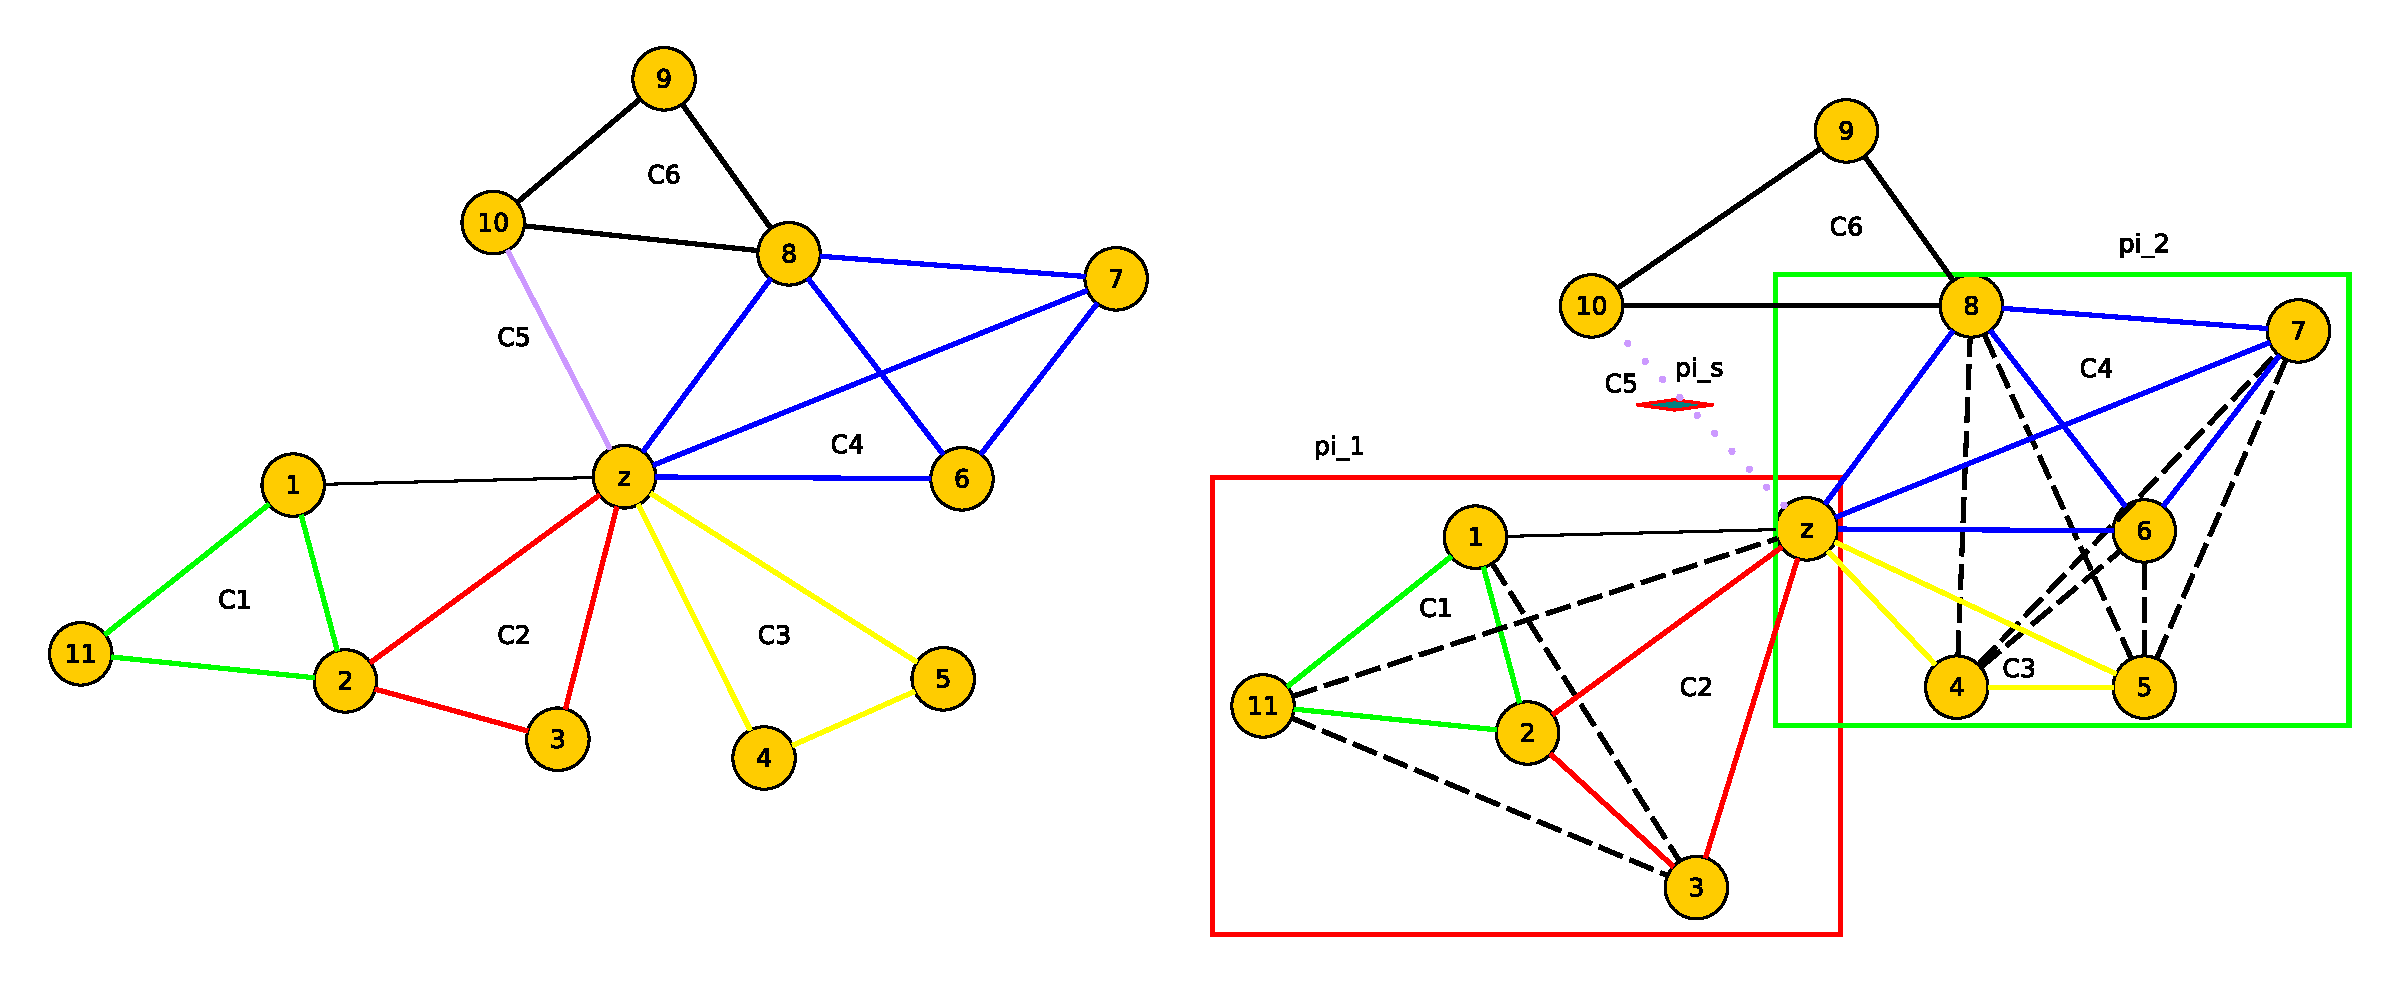
\includegraphics[scale=0.450]{./correctionGraph.eps} \vspace{-0.5em}
\caption{(a) Le sommet $z$ et son voisinage avec les cliques qui le couvrent , (b) un exemple de compression de cliques :  les sommets \`a l'int\'erieur des rectangles rouges et verts forment les nouvelles cliques couvrant $z$.
		$\pi_1 = \{1,2,3,z,11\}$, $\pi_2 = \{z,4,5,6,7,8\}$, $\pi_s = \{10\}$ 
		}
\label{exempleAlgoCorrectionGraphe}
\end{figure}
%% ------ figure correctionGraph
\FloatBarrier

Soient $\pi_1$, $\pi_2$ une bipartition du voisinage du sommet $z_i$  en cliques  et 
$\pi_s$ un ensemble  de sommets dont l'ar\^ete form\'ee par un de ces sommets et le sommet $z_i$ sont  \`a retirer du graphe $G_c$.  
\begin{definition}
Soient 
${\cal CC}^{i}$ la couverture de corr\'elation apr\`es le traitement des $(i-1)^{ieme}$ sommets de ${\cal C}$ et
${\cal CC}^{i}(z_i)$ l'ensemble des cliques contenant le $i^{ieme}$ sommet $z_i$.
\newline
On appelle {\bf compression} du sommet $z_i$ un triplet ($\pi_1$, $\pi_2$, $\pi_s$) d\'efini par : 
\begin{itemize}
	\item $\pi_1$ (resp. $\pi_2$) peut \^etre d'une des formes suivantes :
	\begin{enumerate}
		\item L'union de $z_i$, d'un sous-ensemble $C_1$ (resp. $C_2$) de cliques de ${\cal CC}^{i}(z_i)$ telle que toute paire $(C,C')$ de $C_1$ (resp. $C_2$) est contractable et d'un sous-ensemble $S_1$ (resp. $S_2$) de sommets $v \in S(z_i)$ n'appartenant \`a aucune clique de $C_1$ (resp. $C_2$) tel que
		$$ \forall v \in S_1,~\forall x \in C_1, \not\exists C' \in {\cal CC}^{i}~t.q.~card(C')>2~~et~~\{v,x\} \subset C'$$
		(ce qui fait que \{v,x\} peut \^etre une clique de ${\cal CC}^{i}$).
		\item Une augmentation du sommet $z_i$.
	\end{enumerate}
	\item L'intersection entre $\pi_1$ et $\pi_2$ est r\'eduite $\{z_i\}$ ($\pi_1 \cap \pi_2 = \{z_i\}$),
	\item $\pi_s=\Gamma_{G_c}(z_i)-~((\pi_1 \cap \Gamma_{G_c}(z_i) ) \cup(\pi_2 \cap \Gamma_{G_c}(z_i) ))$ tel que l'ensemble des ar\^etes  $\{[z_i,v]\in E_{c}^{i}:~v\in \pi_s\}$ n'est pas d\'econnectant.
	\item Le triplet $\pi_{1} \cap \Gamma_{G_c}(z_i)$, $\pi_{2} \cap \Gamma_{G_c}(z_i)$, $\pi_{s} \cap \Gamma_{G_c}(z_i)$  est une 3-partition de $\Gamma_{G_c}(z_i)$.
\end{itemize}
\end{definition}
Il existe toujours une telle compression, ne serait-ce que 
$\pi_1 = \{z_i\} \cup C_i \in C(z_i)$, 
$\pi_2 =  \emptyset$,
$\pi_s = \Gamma_{G_c}(z_i) -(\Gamma_{G_c}(z_i) \cup C_i) $  si ${\cal CC}^{i}(z_i)$ n'est pas vide.
Sinon, 
$\pi_1 = \{z_i\} \cup \{ v \in \Gamma_{G_c}(z_i)  \} $, 
$\pi_2 =  \emptyset$,
$\pi_s = \Gamma_{G_c}(z_i) - \{v\} $
est aussi une compression.
Un exemple de compression est aussi donn\'e dans la figure \ref{exempleAlgoCorrectionGraphe}.
Le co\^ut $c(T)$ d'une compression $\pi_{1},\pi_{2},\pi_{s}$ est d\'efini par : 
$$c(T) = | \{\{u,v\} \in \pi_{1}:~[u,v]\not\in E_{c}^{i}\}| + |\{\{u,v\} \in \pi_2:~[u,v]\not\in E_{c}^{i}\}| +~ |\pi_s| $$
%Dans l'exemple de la figure \ref{exempleAlgoCorrectionGraphe}(b), autour d'un sommet $z_i$, l'ensemble $C(z_i)$ contient les cliques $C2$, $C3$,$C4$ et $C5$.
%Les cliques $C5$ et $C4$ ne sont pas contractables, \`a cause de l'existence de $C6$ dans ${\cal C}_i$.
%La clique $C1$ est voisine de $z_i$ et $D_{z_i}(C1) = \{C2\}$.
L'exemple de la compression donn\'ee dans la figure \ref{exempleAlgoCorrectionGraphe}(b) est $\pi_1 = C1 \cup C2$ (une augmentation), $\pi_2 = C3 \cup C4$ (ces deux cliques \'etant contractables), et $\pi_s = \{10\}$.
Les cliques $C1$ et $C2$ sont compress\'ees en ajoutant les ar\^etes $[1,3]$ et $[z_i,11]$. De m\^eme, les cliques $C3$ et $C4$ sont compress\'ees en ajoutant les ar\^etes  $[4,8]$, $[5,8]$, $[7,4]$, $[7,5]$, $[6,4]$ et $[6,5]$. La clique $C5$ est supprim\'ee afin que $z_i$ ne soit pas couvert par trois cliques.
Le co\^ut  de cette compression est $10$, $10$ \'etant le nombre d'ar\^etes en pointill\'ees plus l'ar\^ete supprim\'ee $[10,z_i]$.
\newline

Soit  $c(T)$ le co\^ut minimum d'une compression $T$ de $z_i$.
Le but est de modifier $G_c$ afin que $z_i$ puisse \^etre couvert par une ou deux cliques issues de $\pi_1$ et $\pi_2$.
Pour cela, le co\^ut de cette modification $c(T)$ tient compte des ar\^etes \`a ajouter (li\'ees \`a $\pi_1$ et $\pi_2$) et \`a supprimer (li\'ees \`a $\pi_s$).
\begin{equation}
c(T) = \sum_{ \{u,v\} \subseteq \pi_1: [u,v] \notin E_c^i } \phi^{+}(u,v) + \sum_{ \{u,v\} \subseteq \pi_2: [u,v] \notin E_c^i } \phi^{-}(u,v) + \sum_{ v \in \pi_s } \phi^{-}(u,v)
\end{equation}
Avec $\phi^{+}$ le co\^ut de l'op\'eration {\em ajouter une ar\^ete} et  
$\phi^{-}$ le co\^ut de l'op\'eration {\em ajouter une ar\^ete}.
\newline
Nous \'evaluons les performances des diff\'erents couples de fonctions $\phi^{+}$ et $\phi^{-}$ dans le chapitre \ref{chapitreEvaluation}.
\newline

Ainsi, {\bf appliquer une compression} $T = \pi_1, \pi_2, \pi_s$ consiste \`a ajouter dans $E_c^i$ les ar\^etes d\'efinies par les ensembles de paires $\{\{u,v\} \in \pi_1:~[u,v]\not\in E_{c}^{i}\}$ (qui seront couvertes par la clique $\pi_1$) et $\{\{u,v\} \in \pi_2:~[u,v]\not\in  E_{c}^{i}\}$ (qui seront couvertes par la clique $\pi_2$) et \`a supprimer les ar\^etes $\{[z_i,v] \in  E_{c}^{i}:~v\in \pi_S\}$. 
\newline
D\`es lors, le sommet $z_i$ appartient aux deux cliques $\pi_1$ et $\pi_2$.
On proc\`ede alors aux mises \`a jour suivantes pour obtenir ${\cal CC}^{i+1}$ et $E_M^{i+1}$ :
\begin{itemize}
\item Supprimer toutes les cliques ${\cal CC}^{i}(z_i)$ couvertes par $\pi_1$ dans  ${\cal CC}^{i}$.
\item Supprimer toutes les cliques ${\cal CC}^{i}(z_i)$ couvertes par $\pi_2$ dans  ${\cal CC}^{i}$.
\item Supprimer toutes les cliques de cardinalit\'e $2$ couvertes par $\pi_1$ et $\pi_2$ dans  ${\cal CC}^{i}$.
\item Ajouter $\pi_1$ et $\pi_2$ dans ${\cal CC}^{i}$, supprimer de $E_c^{i+1}$ toutes les ar\^etes  $\{[z_i,v] \in E_c^{i}:~v\in \pi_s\}$.
\item Affecter $Cliq(z)$ \`a $1$ (si $\pi_1$  ou $\pi_2$ est vide) ou $2$ (sinon).
\end{itemize}
Cette proc\'edure a les propri\'et\'es suivantes :
\begin{property}
Consid\'erons l'application d'une compression.\newline
Soit ${\cal CC}^{i+1}$  l'ensemble obtenu \`a partir de ${\cal CC}^{i}$ apr\`es  la mise \`a jour selon cette application.
\begin{itemize}
	\item Tout sommet de $G_c$ couvert par une ou deux cliques dans ${\cal CC}^{i}$ le reste dans ${\cal CC}^{i+1}$.
	\item Toute ar\^ete couverte par une et une seule clique dans ${\cal CC}^{i}$ et qui n'est pas supprim\'ee le reste dans ${\cal CC}^{i+1}$.
	\item Le sommet $z_i$ est couvert par une ou deux cliques dans ${\cal CC}^{i+1}$ (le nombre de sommets ainsi couverts augmente de $1$ par rapport \`a celui dans ${\cal CC}^{i}$).
\end{itemize}
\end{property}

Ainsi, pour chaque sommet $z_i$, on consid\`ere une compression de co\^ut minimum $c_m^i$ et on l'applique.
La propri\'et\'e ci-dessus garantit qu'\`a la fin du processus, on obtient un graphe de corr\'elation $G_c^t = (V_c, E_c^t)$ dont l'ensemble ${\cal CC}^{i}$ modifi\'e est une couverture de corr\'elation.
Consid\'erons la distance de correction $DC(G_c^0, G_c^t ) = | (E_c^0 \cup E_c^t)  - (E_c^0 \cap E_c^t) |$ qui est le nombre de cases modifi\'ees dans la matrice d'adjacence du graphe $G_c$.
La distance-line v\'erifie  
$$DL( G_{c}^{0}, G_{c}^{t}) \le  DC(G_c^0, G_c^t ) $$
Notons que lors d'une \'etape $j > 1$, le sommet $z_j$ et son voisinage se retrouvent \^etre couvert par une ou deux cliques suite au traitement des $j-1$ sommets pr\'ec\'edents, aucune compression ne lui est appliqu\'ee (on consid\`ere la compression identit\'e) et donc 
$c_{m}^{j} = 0$.

	%------- Complexite algorithmes -----------------------------------------------
	\subsection{Complexit\'e des algorithmes}
		L'algorithme de correction traite au plus une fois chaque sommet du graphe.
La complexit\'e de traitement de chaque sommet est exponentielle en fonction du degr\'e de chaque sommet et des cliques auxquelles il appartient, la encore en fonction  de son degr\'e en taille et en nombre.
L'algorithme global (couverture et correction) est donc pseudo-polynomial en fonction du degr\'e du graphe.
\newline

Nous d\'eterminons une conjecture sur le comportement de l'algorithme.
\'Etant donn\'e un graphe de d\'epart, une ex\'ecution de l'algorithme est un ordre dans lequel seront trait\'es les sommets dans l'algorithme de couverture, puis
la s\'election des sommets $z_i$ \`a traiter dans  $\cal C$.
\newline
Consid\'erons un graphe de corr\'elation $G_c$ n'\'etant pas isomorphe \`a un graphe de la figure \ref{graphe2Couverture}. On dira que $G_c$ est non-ambigu.

Deux ar\^etes $[u,v]$ et $[u',v']$ de $G_c$ seront dit {\bf clique-independantes} si et seulement si il n'existe pas de cliques $C$ dans la couverture de corr\'elation  de $G_c$ telle que 
$C \cap \{u,v\} \cap \{u',v'\} \ne \emptyset$

\begin{conjecture}
Si $G'=(V, E')$ est un graphe obtenu en supprimant un ensemble d'ar\^etes deux \`a deux clique-independantes d'un graphe de corr\'elation non-ambigu $G_c = (V,E_c)$, alors il existe une ex\'ecution de l'algorithme qui transforme $G'$ en $G_c$.
\end{conjecture}


	%------- Conclusion description algorithmes -----------------------------------------------
	\subsection{Conclusion de la description des algorithmes}
		% --- a supprimer ce commenntaire cest une redite de l'algorithme de couverture
%Dans cette section, nous d\'ecrivons deux algorithmes. 
%Le premier algorithme est {\em l'algorithme de couverture} et il est bas\'e sur l'algorithme de Lehot \cite{decompositionEnCliques}. L'algorithme consid\`ere que chaque sommet peut avoir $4$ \'etats. Le premier \'etat $Cliq = 1$ est attribu\'e \`a des sommets couverts par une clique ou deux cliques et qui n'a aucune ar\^ete incidente. Le second \'etat $Cliq = 2$ est attribu\'e \`a des sommets couverts par une clique et qui poss\`ede des ar\^etes incidentes. Le troisi\`eme \'etat $Cliq = 3$ est attribu\'e \`a des sommets initialement n'ayant aucun \`etat ($Cliq=0$) et couvert par une clique. Et  le dernier \'etat $Cliq = -1$  est attribu\'e \`a des sommets couverts par deux cliques ayant des ar\^etes incidentes ou un sommet ayant des ar\^etes incidentes qui ne forme pas une clique. 
%\`A la fin de l'algorithme, les cliques d\'ecouvertes sont stock\'ees dans la line-couverture $\cal H$ et les sommets dont l'\'etat est $Cliq = -1$ sont contenus dans l'ensemble $\cal C$ des sommets \`a corriger.


Dans cette section, nous d\'ecrivons deux algorithmes. 
Le premier algorithme est {\em l'algorithme de couverture} qui attribue un \'etat \`a un sommet du graphe de corr\'elation en fonction des cliques qui le couvrent. L'ensemble de cliques est la couverture de corr\'elation ${\cal CC}$. La particularit\'e de la couverture de corr\'elation est que chaque sommet appartient \`a $1$ ou $2$ cliques. Lorsqu'un  sommet  n'est pas couvert par $1$ ou $2$ cliques, cela signifie que le graphe de corr\'elation n'est pas un line-graphe et ces sommets sont regroup\'es dans l'ensemble $\cal C$ de sommets \`a corriger.
\newline
%Le second algorithme present\'e est l'algorithme de correction dont l'objectif est de corriger les sommets de l'ensemble de sommets \`a corriger afin que $G_c$ devient le line-graphe le plus proche possible du DAG. La correction consiste \`a ajouter et supprimer des ar\`etes  incidentes \`a chaque sommet de sommets de tel sorte que la clique retenue soit de co\^ut minimum. Nous supposons que les co\^ut des op\'erations {\em ajouter une ar\^ete} et {\em supprimer une ar\^ete} sont connues.



Le second algorithme est {\em l'algorithme de correction}. Il consiste \`a ajouter ou \`a supprimer des ar\^etes au voisinage d'un sommet $u \in {\cal C}$ afin que la partition de ce sommet et son voisinage forme deux cliques. Pour assurer ces op\'erations d'ajout et de suppression, il utilise une phase d'augmentation et de compression. 
En effet, la phase d'augmentation d\'etermine les cliques de ${\cal CC}$ contenant $u$, les cliques de ${\cal CC}$  dont $u$ partage une ar\^ete avec un sommet de la clique (cliques voisines), les cliques contractables (cliques de ${\cal CC}$ dont l'intersection retourne le sommet $u$) et les cliques d\'ependantes (cliques contenant $u$ dans lesquelles un des sommets partagent une ar\^ete avec une clique de la couverture de corr\'elation ${\cal CC}$). 
Puis elle effectue le produit cart\'esien de ces ensembles de cliques. Chaque \'el\'ement de ce produit est not\'e $\pi_1$ ou $\pi_2$.
Quant \`a la phase de compression, elle s\'electionne deux \'el\'ements du produit cart\'esien qu'elle note  $\pi_1$ et $\pi_2$, puis elle ajoute des ar\^etes \`a  $\pi_1$ et $\pi_2$ dans l'ensemble des ar\^etes initiales du graphe de correction pour en faire des cliques. Elle cr\'ee aussi l'ensemble $\pi_s$ des ar\^etes \`a supprimer pour que le sommet $u$ ne soit couvert que par deux cliques. 
Les cliques $\pi_1$ et $\pi_2$ sont ajout\'ees \`a la couverture de corr\'elation ${\cal CC}$. 
\newline
Avec la d\'ecouverte de la couverture de corr\'elation ${\cal CC}$, nous allons construire le graphe racine de ce line-graphe dans la section suivante.




%--------------------------------------------------------------------
%------- 		graphe root		---------------------
%--------------------------------------------------------------------
\section{D\'etermination de la topologie du r\'eseau \'energ\'etique}
	Soient ${\cal CC}(G_c)$, l'ensemble des cliques du line-graphe $G_c$ et 
le graphe non orient\'e $G'=(V',E')$ sous-jacent du DAG $G$.

Nous consid\'erons que chaque clique de ${\cal CC}(G_c)$ est un sommet dans $G'$.
Si l'intersection de deux cliques $c_1, c_2 \in {\cal CC}(G_c)$ retourne l'ar\^ete $a_i$  alors nous ajoutons  l'ar\^ete $a_i $ dans $E'$ entre les sommets  $c_1, c_2 \in G'$.
Dans  le cas o\`u un sommet de  $G_c$ n'appartient qu'\`a une seule clique $c \in {\cal CC}(G_c)$, nous ajoutons  un nouveau sommet (not\'e $ext\_c$) dans $V'$ puis nous ajoutons une ar\^ete $[ext\_c, c]$ dans $E'$.
Nous obtenons le graphe $G'$ non orient\'e connexe.
Nous utilisons la figure \ref{ExempleGraphesRacinesIsomorphes} pour illustrer la construction de $G'$.
La couverture de corr\'elation de $G_c$ est ${\cal CC}(G_c) = [
 c_1 = \{\{a,b\},\{b,c\},\{b,d\}\}, 
 c_2=\{  \{d,f\},\{f,h\},\{c,f\} \}, 
 c_3 = \{  \{b,c\},\{c,e\},\{c,f\} \}, 
 c_4 = \{  \{c,e\},\{e,g\} \}, 
 c_5 = \{  \{b,d\},\{d,f\} \}]$.
Les sommets du $G'$ sont $V' = \{c_1, c_2, c_3, c_4, c_5\}$.
L'intersection des cliques ci-dessous est non vide et le sommet d'intersection est l'identifiant d'une ar\^ete dans $G'$.
$$
c_1 \cap c_3 = \{b,c\}, ~ 
c_1 \cap c_5 = \{b,d\}, ~ 
c_3 \cap c_2 = \{c,f\}, ~ 
c_3 \cap c_4 =   \{c,e\}, ~ 
c_2 \cap c_5 = \{d,f\}
$$
Pour les sommets de $G_c$ couverts par une seule clique, nous cr\'eons le sommet $ext\_x$ dans $G'$ avec $x$ le nom d'une clique de ${\cal CC}(G_c)$ 
puis nous ajoutons une ar\^ete entre le sommet $ext\_x$ et le sommet de $G'$ correspondant \`a la clique.
Par exemple le sommet $\{a,b\}$ de $G_c$ est couvert par la clique $c_1$. 
Nous relions $ext\_c_1$ de $G'$ avec le sommet $c_1$ de $G'$. 
Nous r\'ep\'etons la m\^eme op\'eration pour les sommets  $\{f,h\}$, $\{e,g\}$ de $G_c$.
Le graphe $G'$ (figure \ref{ExempleGraphesRacinesIsomorphes}(c)) est ainsi construit et est isomorphe au graphe $G$ de la figure \ref{ExempleGraphesRacinesIsomorphes}(a).
% ---- figure graphes racines isomorphe
\begin{figure}[htb!] 
\centering
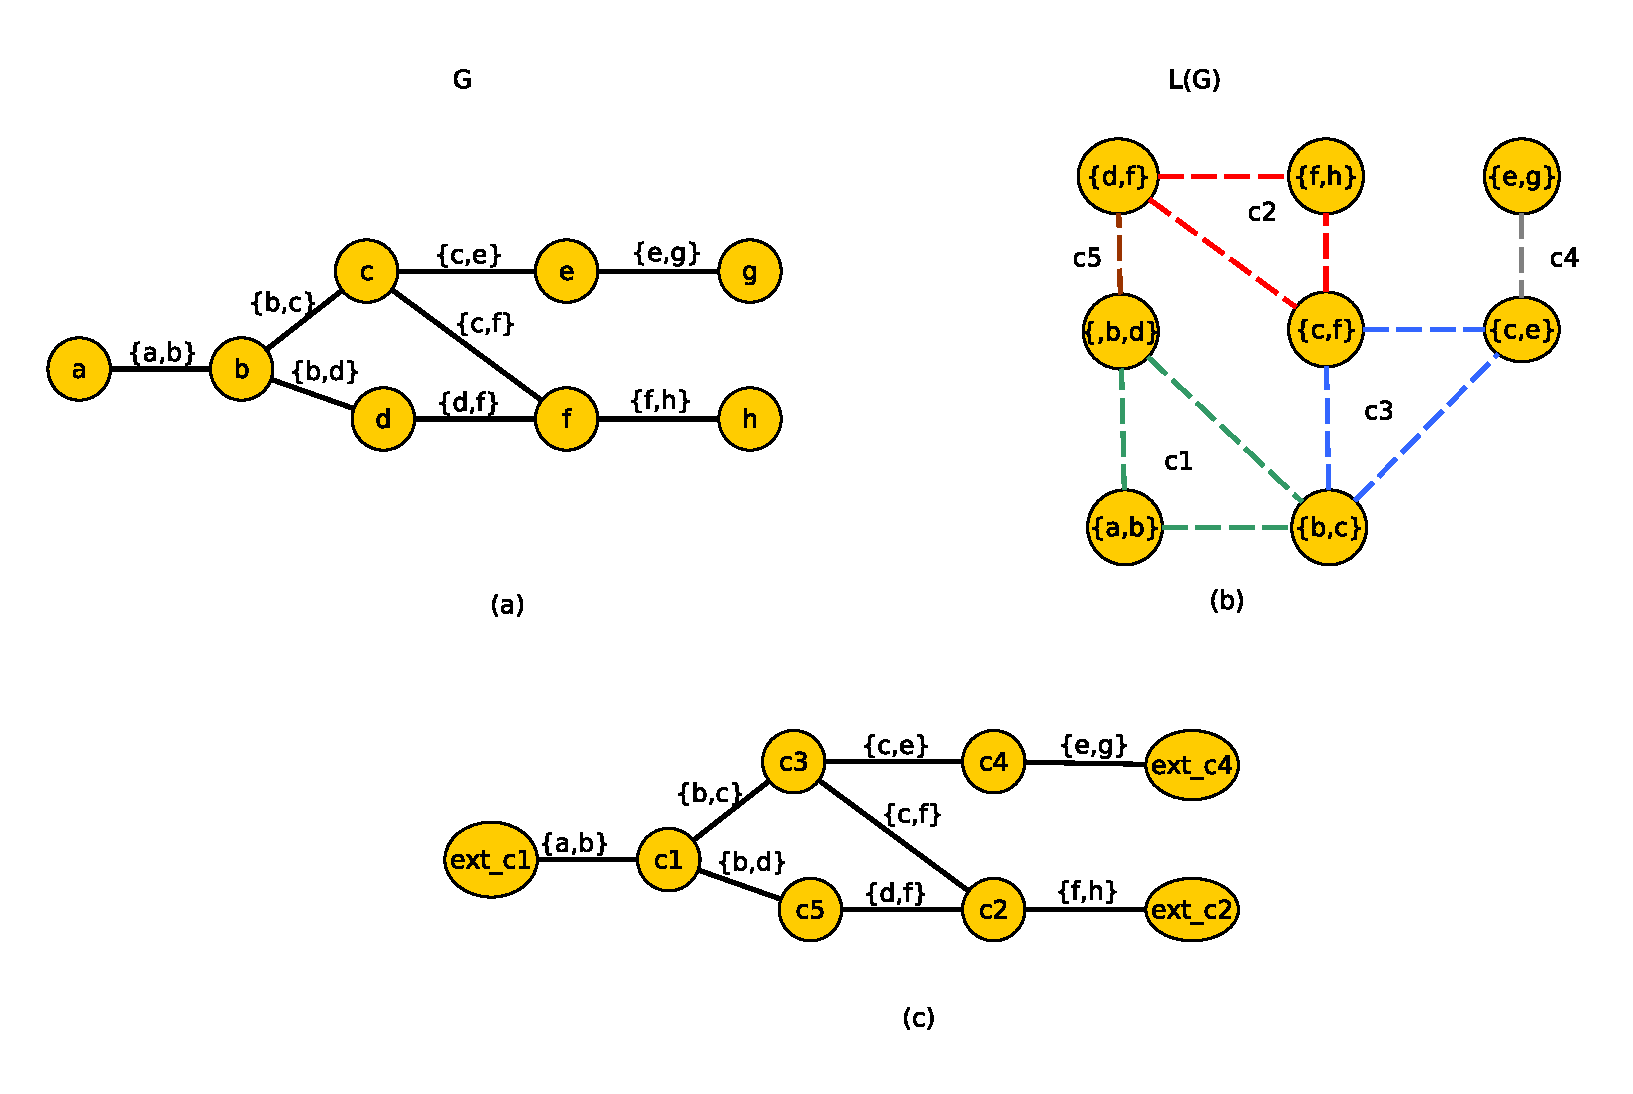
\includegraphics[scale = 0.7]{ExempleGraphesRacinesIsomorphes.eps}
\caption{ Construction de la topologie non orient\'e de $G_c$.
		(a) : r\'eseau initial mod\'elis\'e par $G$.
		(b) : line graphe de $G$.
		(c) : graphe $G'$ reconstruit.
		 }
\label{ExempleGraphesRacinesIsomorphes}
\end{figure}
%\FloatBarrier
% ---- figure exemple correction graphe cellule G_{3,3}

\subsection{Orientation du graphe $G'$}
Nous supposons que le graphe non orient\'e $G'=(V',E')$ sous-jacent au DAG $G$ a d\'ej\`a \'et\'e  obtenu. Nous orientons les ar\^etes de $G'$ afin de d\'ecouvrir  le DAG cible.
 \newline
 
 Soient 
 un sommet $v$, 
 son voisinage $N(v)$ et 
 une bipartition $p(v)$, $s(v)$ de $v$.
 \newline
 Si $Verif-correl (p(v), s(v)) = 1$ alors la partie $p(v)$ est l'ensemble $p(v)$ des arcs entrants de $v$ et  la partie $s(v)$ est l'ensemble $s(v)$ des arcs sortants de $v$.    
Sinon la bipartition n'est pas la bonne et nous testons une autre bipartition.
Nous testons ainsi dans l'ordre de $2^{d(v)}$ bipartitions avec $d(v) = |N(v)|$ dans le pire des cas,.
\newline
Soit une s\'equence $S = v_1, v_2, \cdots, v_k$ de sommets de $G$ telle que 
chaque ar\^ete est incidente \`a $\{v_1, \cdots, v_k\}$ et que  $\{v_1, \cdots, v_{k-1}\}$ n'a pas cette propri\'et\'e.
\newline
Soit $d_i$ le nombre d'ar\^etes liant $v_i$ \`a un sommet  de $V-\{v_1,\cdots, v_{i-1}\}$.
%On determine la couverture. {\bf bizarre} 
\newline
Nous allons prendre dans l'ordre chaque sommet de la s\'equence $S$ et nous allons traiter ses ar\^etes pour trouver une bipartition correcte.
Si une ar\^ete a d\'ej\`a \'et\'e trait\'ee pour un sommet, elle n'est plus prise en compte dans les ar\^etes incidentes des sommets suivants dans la s\'equence $S$.
Le traitement du sommet $v_i$ n\'ecessite $2^{d_i}$ op\'erations et le nombre total d'op\'erations est alors 
$$
 2^{d_1} + 2^{d_2} + \cdots + 2^{d_k}
$$  
Notre probl\`eme  est de trouver une telle liste telle que cette somme est minimum.
L'heuristique est, \`a chaque \'etape, de choisir le sommet tel que 
le nombre d'ar\^etes incidentes non encore trait\'ees est minimum.
Par exemple, on commence par le sommet $v_1$ comme sommet de degr\'ee minimum. 
\`A chaque \'etape, on prend le sommet $v_i$ tel que son degr\'e $d_{v_i}$ est minimum.
\newline 

\vspace{-0.5cm}
Cependant, cette heuristique n'est pas optimale et voici un contre-exemple illustr\'e par la figure \ref{orientationAretesHeuristiqueContreExemple}. \newline
Soit le graphe $H$ compos\'e de $3$ cliques $K_5$ et d'un sommet $v$ ayant une ar\^ete incidente avec un seul sommet dans chaque clique $K_5$.
Le sommet $v$ est de degr\'e minimum. 
Nous consid\'erons $2$ s\'equences de sommets diff\'erents pour d\'enombrer les bipartitions. 
La premi\`ere s\'equence suit l'heuristique et la seconde s\'equence d\'ebute par un sommet de $K_5$ de degr\'e $4$. 
\newline
Soit $c(S)$ la somme des bipartitions possibles.  
En consid\'erant l'heuristique, nous d\'ebutons par $v$. 
Puis le sommet suivant de degr\'e minimum est un sommet de $K_5$. On traite tous les sommets de cette clique $K_5$ avant de passer \`a une autre clique $K_5$.
Le nombre de bipartitions trait\'ees avec  l'heuristique est 
$$
	c(S_H) = 2^3 + 3(  2^4 + 2^3+ 2^2 +2^1) = 98
$$
En consid\'erant la seconde s\'equence, on choisit le sommet de $K_5$ de degr\'e minimum. On traite ce sommet en $2^4$ bipartitions. Le sommet suivant est encore dans cette clique mais le nombre de bipartitions baisse \`a $2^3$.
Apr\`es les deux sommets trait\'es, le nombre de bipartitions est $2^4+2^3$.
On r\'ep\`ete le traitement des sommets jusqu'\`a ce que tous les sommets soient trait\'es avant de passer \`a une autre clique $K_5$. 
Dans cette clique, on reprend \`a nouveau la seconde s\'equence.
Le nombre de bipartitions  trait\'ees avec la seconde s\'equence est 
$$
	c(S_2) = 3(  2^4 + 2^3+ 2^2 +2^1) = 96
$$
Nous remarquons que le nombre de bipartitions avec la seconde s\'equence est minimum.
Cet exemple confirme que la solution de l'heuristique n'est pas minimale car il existe une autre s\'equence de choix de ces sommets (ici la seconde  s\'equence) qui minimise le nombre de bipartitions. 
% ---- figure contre exemple  heuristique orientation aretes 
\begin{figure}[htb!] 
\centering
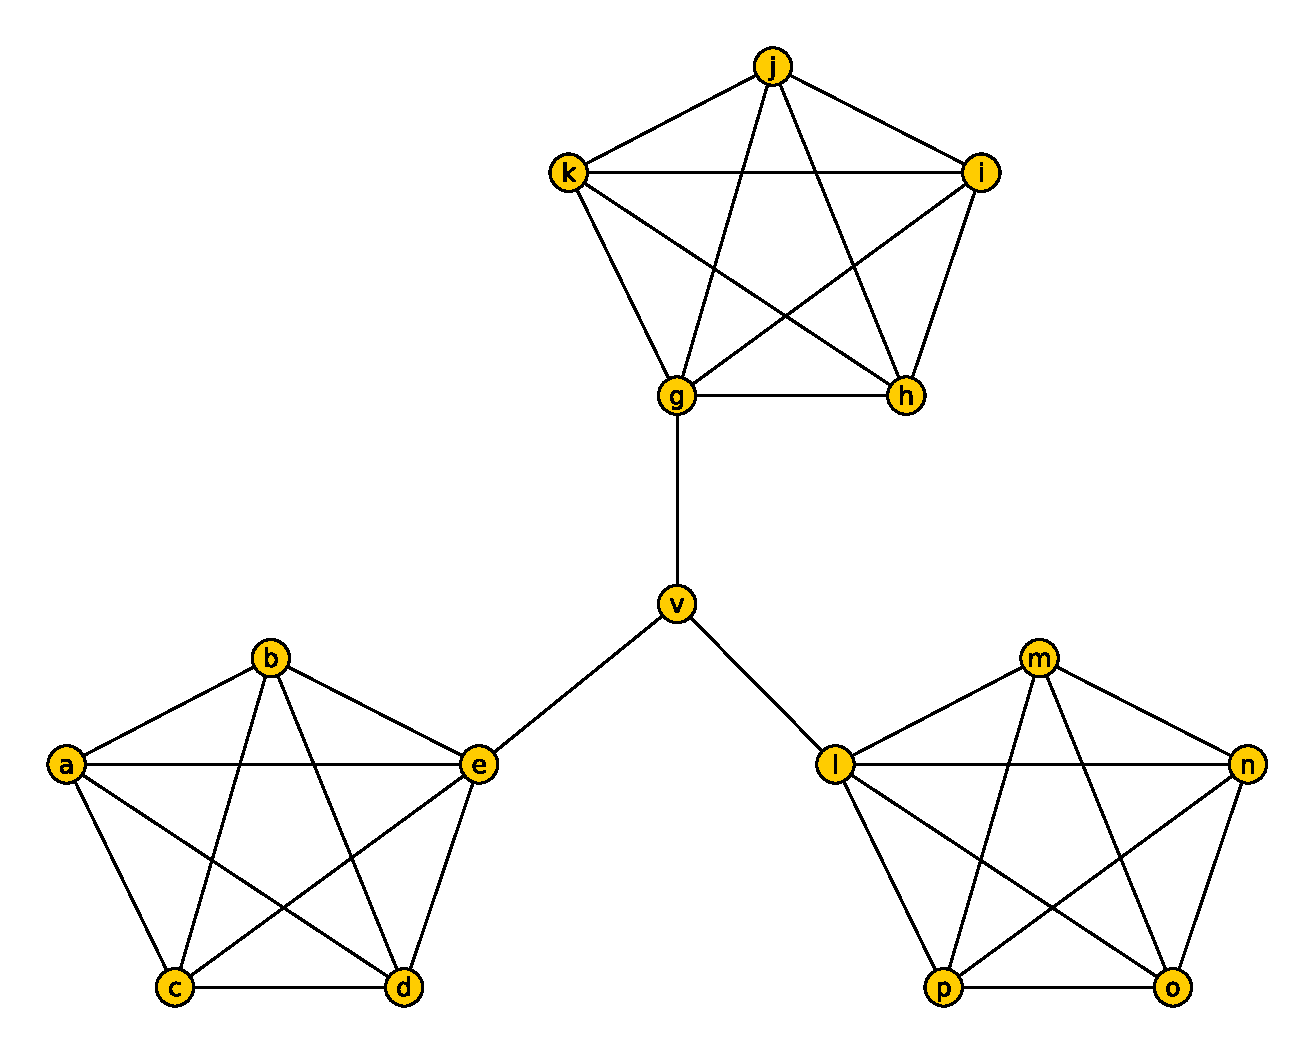
\includegraphics[scale = 0.7]{orientationAretesHeuristiqueContreExemple.eps}
\caption{ Un contre-exemple de l'heuristique choisie pour l'orientation des ar\^etes.
		 On choisit un sommet de degr\'e minimum dans une clique $k_5$. Ensuite, on traite tous les sommets de la clique et on se sert du degr\'e minimum pour choisir les sommets de la s\'equence. Puis on passe \`a une clique et on reprend le traitement jusqu'\`a ce qu'il ne reste plus d'ar\^etes dans une seule clique.
		}
\label{orientationAretesHeuristiqueContreExemple}
\end{figure}
\FloatBarrier
% ---- figure contre exemple  heuristique orientation aretes
%\newline

{\bf Conclusion} : 
l'algorithme d'orientation que nous avons propos\'e choisit le sommet de degr\'e minimum \`a chaque \'etape de l'algorithme et cette solution n'est pas optimale.
Nous conjecturons que la s\'equence $S$ de traitement des sommets est $NP-complet$.


%On le traite avec  $2^3$ bipartitions. Ensuite le sommet suivant de degr\'e minimum est un sommet de $K_5$. On le traite en $2^4$ bipartitions      
%
%
%
%
%Nous supposons que le graphe non-orient\'e $G'=(V',E')$ sous-jacent au DAG $G_c$ ait d\'ej\`a \'et\'e construite. Nous orientons les ar\^etes de $G'$ afin qu'il soit un DAG.
% \newline
% 
%Soit $O = (v_1,v_2, \cdots, v_n)$ la s\'equence de traitement des sommets de $G'$ tel que 
%$d_1 \le d_2 \le \cdots \le d_n$ avec 
%$d_i$ le degr\'e du sommet $v_i$. $d_i$ est aussi le le nombre d'ar\^etes incidentes \`a $v_i$ non trait\'es.
%\newline
%Consid\'erons le premier sommet $v_1$ \`a traiter de $O$ et $N(v_1)$ l'ensemble des  ar\^etes incidentes \`a $v_1$.
%Nous subdivisons $N(v_1)$ en $2$ partitions telles que 
%\begin{itemize}
%	\item $pred(v_1)$ est l'ensemble des ar\^etes pr\'ed\'ecesseurs \`a $v_1$.
%	\item $succ(v_1)$  est l'ensemble des ar\^etes successeurs \`a $v_1$.
%\end{itemize}
%Nous testons cette bipartition $(pred(v_1), succ(v_1))$ avec la fonction $Verif-correl$ \ref{VerifCorrel}.
%Si $Verif-correl$ retourne $Vrai$ alors nous avons orient\'e les ar\^etes incidentes \`a $v_1$.
%Sinon nous testons une autre bipartition.
%Dans le pire des cas, nous testons $2^{d_1}$ bipartitions pour trouver la bonne.
%\newline
%Soit  $(pred(v_1), succ(v_1))$ la bonne bipartition de $v_1$.
%\'Etant donn\'ee que $G'$ est un graphe connexe et que une ar\^ete $a_i$ est form\'ee par les sommets $v_i$ et $v_j$ de $G'$, 
%$a_i$ appartient \`a l'ensemble des successeurs de $v_j$ si $a_i$ a d\'ej\`a \'et\'e trait\'e en pr\'ed\'ecesseur de $v_i$.
%De m\^eme, $a_i$ appartient \`a l'ensemble des pr\'ed\'ecesseurs de $v_j$ si $a_i$ a d\'ej\`a \'et\'e trait\'e en successeur de $v_i$.
%Ainsi, le nombre de bipartitions \`a tester devient moins important au traitement d'un nouveau sommet de $O$.
%En effet, le nombre de bipartitions \`a tester en traitant le sommet  $v_2$ est $2^{d_2}$ et $2^{d_2} \le 2^{d_1}$.
%En traitant le dernier sommet $v_n$ de $O$, nous testons une seule bipartition parce que tous les ar\^etes ont d\'ej\`a \'et\'e trait\'es. Cette bipartition est la bonne et $2^{d_n} = 1$.
%\newline
%Nous d\'eduisons que 
%$$
%1 = 2^{d_n} \le \cdots \le 2^{d_2} \le 2^{d_1}
%$$
%
%L'algorithme d'orientation que nous avons propos\'e choisit le sommet de degr\'e minimum \`a chaque \'etape de l'algorithme et cette solution est minimale.
%Nous conjecturons que la s\'equence $O$ de traitement des sommets est $NP-complet$.
%
%
%
%%% ----
%%% decouverte de topologie du reseau energetique
%%% ----
%%Soient $\cal H$, l'ensemble des cliques de la line-graphe $G_c$ et $G$ le graphe racine de $G_c$. \newline
%%Chaque clique $C_k \in {\cal H}$ correspond \`a un sommet du graphe racine $G$. \newline 
%%Soit $u = \{ENTRANT, SORTANT, NONE\}$, l'ensemble des marquages de chaque ar\^ete tel que les \'etiquettes {\em ENTRANT} et {\em SORTANT} sont associ\'ees respectivement \`a l'ar\^ete $a_i$ entrante et \`a l'ar\^ete $a_j$ sortante du sommet $C_k$.
%%\newline
%%%-- definition de S_1 e S_2
%%Soient $S_1$ et $S_2$ l'ensemble des arcs entrants et sortantes du sommet $C_k$.
%%\begin{equation}
%%S_\alpha = \{ S_{\alpha,i}, \hspace{0.2 em} \forall i \le 2^{card(C_k)+1}  \}
%%\end{equation}
%%avec $i$, le nombre de sous-ensemble de $C_k$ et $\alpha = \{1,2\}$. Le sous-ensemble $S_{\alpha,i}$ peut \^etre  l'ensemble vide $\emptyset$.
%% 
%% %--  ORACLE ou Verif-correl
%% \begin{definition}
%% Soit la clique $C_k$ de la line-couverture {\cal H}.
%% Un couple $(S_1,S_2)$ de sous-ensembles de $C_k$ est {\bf valide} si 
%% \begin{itemize}
%% \item $S_1 \ne S_2$
%% \item $S_1 \cup S_2 = C_k$
%% \item $S_1 \cap S_2 = \emptyset$
%% \end{itemize}
%% \end{definition}
%% 
%% \begin{definition}
%% Soit une fonction bool\'eenne $Verif-correl$ d\'efinit de $S_1 \times S_2 \rightarrow \{0,1\}$, avec le couple valide $(S_1,S_2)$.
%% La fonction $Verif-correl$ renvoie $1$ si et seulement si la loi de conservation autour du sommet $C_k \in G$ est respect\'ee c'est-\`a-dire : 
%% \begin{equation}
%% \forall a_i \in S_1, \forall a_j \in S_2, \sum_{a_i \in S_1} gp_{a_i} - \sum_{a_j \in S_2} gp_{a_j} \le \epsilon
%% \end{equation}
%% avec $\epsilon$ les pertes minimales par effets joules, $gp_{a_i}$ le flot dans l'arc $a_i \in E(G_c)$.
%% \end{definition}
%% 
%% \begin{property}
%% Si $Verif-correl(S_1, S_2) = 1$ alors l'ensemble  $S_1$ est l'ensemble des arcs entrants et  $S_2$ l'ensemble des arcs sortants du sommet $C_k \in G$.
%% \end{property} 
%%Les arcs de $S_1$ et $S_2$ ne concourent pas \`a un sommet $C_k$ lorsque  $Verif-correl(S_1, S_2) = 0$.
%%
%%\begin{theorem}
%%\label{arcsentrantsSortants}
%%%Un arc $a_i$ est soit {\em entrant}, soit {\em sortant} mais jamais les deux.
%%Si un sommet $a_i \in G_c$ appartient \`a deux cliques $C_{k_1}, C_{k_2} \in {\cal H}$ alors 
%%l'arc  $a_i \in E(G_c)$ est soit {\em entrant} de $C_{k_1}$  et {\em sortant} de $C_{k_2}$ ou soit {\em entrant} de $C_{k_2}$  et {\em sortant} de $C_{k_1}$.
%%\end{theorem}
%%
%%\begin{proof}
%%D'apr\`es le th\'eor\^eme \ref{caracteristiquesLinegraphes}, le sommet $a_i$ appartient \`a deux cliques $C_{k_1}$ et $C_{k_2}$ au maximum. 
%%Cela implique qu'il existe une ar\^ete entre les sommets $C_{k_1}$ et $C_{k_2}$ dans $G$.
%%Soient $S_1, S_2 \subset C_{k_1}$ et $S_3, S_4 \subset C_{k_2}$ telles que $Verif-correl(S_1, S_2) = 1$ et $Verif-correl(S_3, S_4) = 1$.
%%Comme  $S_1 \cap S_2 = \emptyset$, $S_3 \cap S_4 = \emptyset$ et aussi  $C_{k_1} \cap C_{k_2} = \{a_i\}$, on a quatre choix possibles :
%%$a_i \in S_1 \cap S_3$, $a_i \in S_1 \cap S_4$, $a_i \in S_2 \cap S_3$, $a_i \in S_2 \cap S_4$.
%%\newline
%%Si $a_i$ est entrant \`a $C_{k_1}$ et sortant \`a  $C_{k_2}$ alors $a_i \in S_1 \cap S_3$ ou  $a_i \in S_2 \cap S_4$. 
%%On en d\'eduit qu'il existe une boucle sur le sommet $C_{k_1}$ et $C_{k_2}$. 
%%Cela est impossible parce que $G$ est un $DAG$. 
%%\newline
%%Ainsi si $a_i$ est entrant \`a $C_{k_1}$ alors $a_i \in S_2 \cap S_3$ ou  si $a_i$ sortant \`a $C_{k_2}$  alors $a_i \in S_1 \cap S_4$. 
%%\end{proof}
%%
%%consid\'erons l'ensemble $A$ des cliques $C_j$ tel que $card(C_j) = min\{ card(C_k), C_k \in {\cal H}\}$ et la fonction  $Z$ qui retourne l'\'etiquette d'un sommet dans une clique. $Z$ est d\'efinie comme suit:
%%$E \times {\cal H} \rightarrow \{ENTRANT, SORTANT, NONE\} $.
%%\newline
%%Soit la fonction $f$ d\'efinie sur $ V(G_c) \times A \rightarrow \{0,1\}$ retournant $1$ si le sommet $a_i^u$ ne poss\`ede aucune \'etiquette c'est-\`a-dire labellis\'e \`a $None$.
%%$$ f(a_i^u, C_j) = \begin{cases} 1 ~~~ si ~~~ Z(a_i^u, C_j) \ne NONE \\ 0 ~~~ sinon \end{cases}$$.
%%La fonction $MA$ calcule le nombre de sommets labellis\'e dans une clique $C_k$.
%%$$MA(C_k) =  \sum_{a_i^u \in C_k} f(a_i^u,C_k) $$
%%Soient la clique $C_m$ telle que  $MA(C_m) = max\{ MA(C_j), C_j \in A\}$ et $B$ l'ensemble des sommets de la clique $C_m$ tel que $Z( a_j^v, C_m) == NONE, ~ \forall ~ a_j^v \in B$. 
%%
%%
%%%nommer l'algorithme
%%\begin{algorithm}[!ht]
%%\caption{Decouverte\_graphe\_racine}
%%\noindent DEBUT\\
%%\noindent 1. Initialisation des \'etiquettes des sommets $a_i$ de $G_c$, et $C_k \in {\cal H}$ \\
%%\noindent $Z( C_k, a_i^u) = None$ \\
%%~2. \indent {\bf Tant que} il existe une  ar\^ete de $G_c$ ($E(G_c)$) \\
%%	\indent~~~~~~{\bf Faire}\\
%%~3.		\indent~~~~~~~~choisir $A = \{C_j , card(C_j) = min\{ card(C_k), C_k \in {\cal H} \}\}$ \\
%%~4.		\indent~~~~~~~~choisir $C_k$ tel que $MA(C_k) = max\{ MA(C_j), C_j \in A\} $ \\
%%~5.       	\indent~~~~~~~~{\bf Si} il existe $S_1$ et $S_2$ tel que $S_1 \cap S_2 = \emptyset $ et $S_1 \cup S_2 = C_k $ et $Verif-correl(S_1, S_2 )= 1 $ \\
%%~6.	       	\indent~~~~~~~~~~~~{\bf alors}\\
%%~7.	       	\indent~~~~~~~~~~~~ $S_1^k = sommets\_marques(S_1, Z)(^1)$; \\
%%~8.	       	\indent~~~~~~~~~~~~ $S_2^k = sommets\_marques(S_2, Z)$; \\
%%~9.		\indent ~~~~~~~~~~~~{\bf Pour tout} $a_i^K \in S_1 - S_1^k$ {\bf Faire} \\
%%~10.		\indent ~~~~~~~~~~~~~ $Z(C_k, a_i^K) = ENTRANT$ \\
%%~11.		\indent ~~~~~~~~~~ {\bf Pour tout} $a_i^K \in S_2 - S_2^k$ {\bf Faire} \\
%%~12.		\indent ~~~~~~~~~~~~~ $Z(C_k, a_i^K) = SORTANT$ \\
%%~13.		\indent~~~~~~~~~~ $E(G_{c}) =  E(G_c)  - E(G_c[C_k])$ \\
%%~14.		\indent~~~~~~~~~~ ${\cal H} =  {\cal H}  - C_k$ \\
%%~15.       	\indent~~~~~~~~{\bf FinSi} \\
%%~16. \indent {\bf FinTant que} \\
%%~17. \indent {\bf Pour tout} $a_i^u \in V(G_c)$ {\bf Faire} \\
%%~18. \indent ~~~ $C_1, C_2$ = $Couverture\_Cliques(a_i^u)(^2)$\\
%%~19. \indent ~~~ {\bf Si } $C_1 \neq \emptyset$ et $C_2 \neq \emptyset$ {\bf Alors} \\
%%~20. \indent ~~~~~~  {\bf Si}  $Z(C_1, a_i^u) == SORTANT$ {\bf Alors} \\
%%~21. \indent ~~~~~~~~~~~~ $Mat(C_1)$ += $C_2$ $(^3)$ \\  
%%~22. \indent ~~~~~~  {\bf Fin Si} \\
%%~23. \indent ~~~~~~  {\bf Si}  $Z(C_2, a_i^u) == SORTANT$ {\bf Alors} \\
%%~24. \indent ~~~~~~~~~~~~ $Mat(C_2)$ += $C_1$ $(^3)$ \\  
%%~25. \indent ~~~~~~  {\bf Fin Si} \\
%%~26. \indent ~~~ {\bf Fin si} \\
%%~27. \indent ~~~ {\bf Si } $C_1 \neq \emptyset$ et $C_2 == \emptyset$ {\bf Alors} \\
%%~28. \indent ~~~~~~  {\bf Si}  $Z(C_1, a_i^u) == ENTRANT$ {\bf Alors} \\
%%~29. \indent ~~~~~~~~~~~~ $Mat(EXT\_a_i^u)$ += $C1$ $(^3)$\\  
%%~30. \indent ~~~~~~  {\bf Fin Si} \\
%%~31. \indent ~~~~~~  {\bf Si}  $Z(C_1, a_i^u) == SORTANT$ {\bf Alors} \\
%%~32. \indent ~~~~~~~~~~~~ $Mat(C_1)$ += $EXT\_a_i^u$ $(^3)$ \\  
%%~33. \indent ~~~~~~  {\bf Fin Si} \\
%%~34. \indent ~~~ {\bf Fin si} \\
%%~35. \indent {\bf Fin Pour} \\
%%~36. \noindent {\bf Return} Mat\\
%%\noindent FIN\\
%%\end{algorithm}
%%
%%\FloatBarrier
%%$^1$ : Cette fonction retourne les sommets de l'ensemble $S_1$ labellis\'es \`a $ENTRANT$ et $S_2$ labellis\'es \`a $SORTANT$. Initialement, Ces sommets sont \'etiquett\'es \`a $NONE$.
%%
%%$^2$ : Cette fonction renvoie les cliques couvrantes une ar\^ete $a_i^u$ avec $C_1 \ne \emptyset$. Si $a_i^u$ est couvert par une clique alors $C_2 = \emptyset$.
%%
%%$^3$ : $EXT\_a_i^u$ est un sommet du graphe racine $G$.
%%\newline
%%
%%L'algorithme {\em Decouverte\_graphe\_racine} d\'ebute par l'initialisation des sommets de $G_c$ \`a $''None''$.
%%Tant qu'il existe une ar\^ete dans notre line-graphe $G_c$, on choisit la plus petite clique $C_k$ dans laquelle le nombre de sommets labellis\'es est maximal quelque soit le label {\em ENTRANT} et {\em SORTANT} (lignes $3-4$).
%%On partitionne la clique $C_k$  en deux sous-ensembles valides $S_1$ et $S_2$ tels que $S_1$ et $S_2$ correspondent, respectivement, \`a l'ensemble des arcs entrants et sortants du graphe racine $G$.
%%Les sommets labellis\'es de $S_1$ not\'es $S_1^k$ portent l'\'etiquette $ENTRANT$ tandis que ceux labellis\'es en $''SORTANT''$ sont not\'es $S_2^k$ (lignes $6-12$). 
%%Ensuite nous mettons \`a jour l'ensemble des ar\^etes et la line-couverture  $\cal C$ de $G_c$ (lignes $13-14$). 
%%\newline
%%Une fois termin\'e l'orientation des ar\^etes de $G$ qui  sont les sommets labellis\'es du line-graphe $G_c$ (lignes $2-16$), nous construisons la liste d'adjacence de chaque sommet de $G$ (lignes $17-36$).
%%Nous recherchons la couverture d'un sommet $a_i^u$ de $G_c$.
%%\newline 
%%Si le sommet  $a_i^u$ est couvert par une seule clique alors $C_2 = \emptyset$. Dans ce cas, cela signifie qu'il existe un arc entre le sommet $C_1$ et le sommet $EXT\_a_i^u$ que nous avons cr\'ee. Cet arc a pour extr\'emit\'e initiale $C_1$ si $a_i^u$ est labellis\'e par $SORTANT$ sinon pour extr\'emit\'e initiale $EXT\_a_i^u$ si $a_i^u$ est labellis\'e par $ENTRANT$ (lignes $27-34$).
%%\newline
%%Dans le cas o\`u le sommet $a_i^u$ est couvert par deux cliques non vides $C_1, C_2$, nous ajoutons un arc entre ces deux cliques.
%%D'apr\'es le th\'eor\`eme  \ref{arcsentrantsSortants}, nous d\'efinissons  $C_1$ comme extr\'emit\'e initiale de cet arc si $a_i^u$ est labellis\'e par $SORTANT$ dans cette clique $C_1$. Dans le cas o\`u $a_i^u$ est labellis\'e par $SORTANT$ dans cette clique $C_2$, $C_2$ est l'extr\'emit\'e finale de cet arc (lignes $19-26$).
%%%D'apr\'es le th\'eor\`eme  \ref{arcsentrantsSortants} stipulant qu'un sommet de $G_C$ est $''ENTRANT''$ de $C_1$ et $''SORTANT''$ de $C_2$ et vice-versa, nous d\'efinissons  $C_1$ comme extr\'emit\'e initiale de cet arc si $a_i^u$ est labellis\'e par $SORTANT$ dans cette clique $C_1$ sinon $C_2$ si $a_i^u$ est labellis\'e par $SORTANT$ dans cette clique $C_2$ (lignes $19-26$).
%%
%%\subsection{Complexit\'e de l'algorithme {\em Decouverte\_graphe\_racine} }
%%
%%La fonction $Couverture\_Cliques$ a une complexit\'e constante $O(1)$ alors que la complexit\'e de la  fonction $sommets\_marques$ depend du nombre de sommets dans $S_1$. Dans le pire des cas, sa complexit\'e est $O(n)$ avec $n = E(G)$ le nombre  d'arcs de $G$. Donc les lignes $17-35$ s'ex\'ecutent en $O(n)$ dans le pire des cas. 
%%\newline
%%Consid\'erons une line-couverture ${\cal H}$  de taille $K$,  une clique $C_i \in {\cal H}$ de taille $p_i$ et $k_i$ le nombre de sommets marqu\'es dans $C_i$. 
%%\newline
%%Le nombre de couples valides $(S_1,S_2)$ pour la clique $C_i$ avec $k_i$ sommets marqu\'es est $2^{p_i -k_i}$. 
%%Au traitement de la premi\`ere clique de ${\cal C}$ de taille minimale $C_1$, il existe $0$ sommet marqu\'e. Le co\^ut $R_{cv_1}$ de couples valides est $R_{cv_1} = 2^{p_1}$.
%%Au traitement de la seconde clique $C_2$, il existe $k_2 \ge 0$ et son co\^ut est  $R_{cv_2} = 2^{p_2 - k_2}$.
%%Il existe une clique $C_\alpha$ \`a partir de laquelle $k_\alpha > 0, \alpha \le K$.
%%On remarque que $p_\alpha - k_\alpha$ est d\'ecroissant car $k_\alpha$ augmente apr\`es chaque traitement de cliques. 
%%Cela signifie qu'\`a la selection de la derni\`ere clique $C_k$, son co\^ut  est de $R_{cv_K} = 1$. 
%%Le co\^ut est decroissant \`a chaque traitement c'est-\`a-dire 
%%$$2^{p_{\alpha} - k_{\alpha}} \ge 2^{p_{\alpha+1} - k_{\alpha+1}} \ge \cdots \ge 2^{p_K - k_K}$$ 
%%Le co\^ut des couples valides de ${\cal H}$ est 
%%$$R_{cv} = O(2^\gamma), \gamma = max\{card(C_i), \forall C_i  \in \{C_1, \cdots, C_\alpha\} \}$$
%%car il depend de la clique $C_i \in \{C_1, \cdots, C_\alpha\} \subset {\cal H}$.
%%\newline
%%Le co\^ut des lignes $3-4$ depend de $p_i$ et $K$ ($O(p_i) + O(K)$) et celui des lignes $7-14$ est de $O(p_i^2)$.
%%\newline
%%Soit le co\^ut $R$ de la boucle  {\em Tant que}. Il est de 
%%$$ R = O(p_i) + O(K) + O(p_i^2) + O(2^\gamma) \simeq O(2^\gamma)$$
%%
%%La complexit\'e de {\em Decouverte\_graphe\_racine} est {\em pseudo-exponentielle} car l'exposant $\gamma$ est la taille d'une clique de taille interm\'ediaire.
%%
%%%Consid\'erons les instructions dans le boucle {\em Tant que}, $K$ le cardinal de ${\cal C}$ et $p$ le cardinal de la clique de taille minimale de ${\cal C}$ c'est-\`a-dire $card(A) = p$. 
%%%\newline
%%%$R_i$ est le co\^ut de la boucle {\em Tant que} au traitement de la $i^eme$ clique de $G_C$ et $C\_oracle$ le co\^ut de la fonction $ORACLE$.
%%%S\'electionnons le premier clique de $G_C$. Son co\^ut est :
%%%$$R_1 = p \times C_oracle(S_{1p}, S_{2p}) $$.
%%%Le co\^ut  du deuxi\`eme sommet est :
%%%$$R_2 = p \times C_oracle(S_{1p}, S_{2p})  + (p-1) \times C_oracle(S_{1p-1}, S_{2p-1})  $$.
%%%Le co\^ut des $n$ sommets de $G_C$ est :
%%%$$R_K = \sum_{k = 0}^{K-1} (p-k) \times C_oracle(S_{1p-k}, S_{2p-k})$$
%%%
%%%La particularit\'e de l'ORACLE est que pour $k \ge p$, tous les sommets de la clique $C_k$ sont labellis\'es entrainant qu'on ne genere aucuns sous-ensembles de $C_k$. Cela implique que  $C_oracle(S_{1p-k}, S_{2p-k}) = 1$. \newline
%%%Cela revient \`a dire que le co\^ut $R_K$ est d\'ecroissant en fonction de $K$. \newline
%%%G\'en\'erer tous  sous-ensembles de $C_k$ de taille $p$ est une combinaison de 
%%%$card(P(E)) = 2^{p}$ et toutes les paires de $P(E)$ vaut au pire des cas $\frac{2^p * (2^p - 1)}{2}$. 
%%%Alors  le  cout  $C_oracle(S_{1p}, S_{2p}$ est $O(2^p)$ ===> FAUX
%%%%%%% A discuter avec SERGES ---> trouver le nombre de tuples provenant des sous ensembles  de C_k de taille $p$
%%%Donc le co\^ut de $R_K$ est  
%%%$$R_K = p \times O(2^p) + (p-1) \times O(2^{(p-1)}) + \cdots + 1 \times O(2^0)$$
%%%$$ R_K $$
%%%PAS FINI
%%
%%

		
%--------------------------------------------------------------------
%------- 	conclusion chapitre		 ---------------------
%--------------------------------------------------------------------
\section{Conclusion du chapitre \ref{linegraphesChapitre} }
	%%% reformulation et correction 
Nous avons d\'ecrit la relation existante entre la matrice de corr\'elation et la notion de line-graphe. En effet, la matrice de corr\'elation appliqu\'ee \`a une valeur de seuil est la matrice d'adjacence d'un line-graphe si elle ne contient aucune erreur de corr\'elation.  Dans le cas o\`u elle poss\`ede des cases \'erron\'ees, il est impossible de d\'eterminer la {\em couverture de corr\'elation} du graphe de corr\'elation. Nous avons alors d\'efini le probl\`eme {\em Proxi-Line} dont l'objectif est de trouver le line-graphe  qui a le moins d'ar\^etes diff\'erentes avec le graphe de corr\'elation.  
\newline

Ensuite, nous avons pr\'esent\'e les propri\'et\'es d'un line-graphe et les travaux existants dans la d\'ecouverte de couverture en cliques sur des line-graphes. Nous avons retenu l'algorithme de Lehot \cite{decompositionEnCliques} comme la base de notre algorithme de couverture parce qu'il attribue  des \'etats \`a tous les sommets \`a chaque \'etape de l'algorithme. Cette op\'eration permet de connaitre les sommets non couverts des sommets d\'ej\`a couverts. 
\newline
Dans le but de r\'esoudre le probl\`eme {\em Proxi-Line}, nous proposons ainsi deux algorithmes. 
\newline
Le premier algorithme est {\em l'algorithme de couverture} et il couvre tous les sommets par une ou deux cliques \`a partir des \'etats des sommets. Nous avons distingu\'e trois types d'\'etats.
En effet, un sommet couvert par une clique et qui poss\`ede des ar\^etes incidentes est \`a l'\'etat  $2$. Un sommet couvert par une clique ou deux cliques et qui n'a aucune ar\^ete incidente est \`a l'\'etat $1$. Un sommet couvert par deux cliques ayant des ar\^etes incidentes ou un sommet ayant des ar\^etes incidentes qui ne forment pas une clique est \`a l'\'etat $-1$. 
L'ensemble des sommets $v$ \`a l'\'etat $-1$ est l'ensemble $\cal C$ de sommets \`a corriger. \`A la fin de l'algorithme, il retourne les cliques d\'ecouvertes (couverture de corr\'elation $\cal CC$). 
\newline
Le second algorithme propos\'e est {\em l'algorithme de correction}. Il se base sur l'ensemble $\cal C$ et les cliques d\'ecouvertes pendant l'algorithme de couverture. 
En effet, cet algorithme s\'electionne chaque sommet $u \in \cal C$ et le corrige en proc\'edant par une phase d'augmentation et de compression.
La phase d'augmentation d\'etermine les cliques de $\cal CC$ contenant $u$, les cliques de $\cal CC$  dont $u$ partage une ar\^ete avec un sommet de la clique (cliques voisines), les cliques contractables (cliques de $\cal CC$ dont l'intersection retourne le sommet $u$) et les cliques d\'ependantes (cliques contenant $u$ dans lesquelles un des sommets partagent une ar\^ete avec une clique de la couverture  de corr\'elation $\cal CC$). 
Puis elle effectue le produit cart\'esien de ces ensembles de cliques. Chaque \'el\'ement de ce produit est not\'e $\pi_1$ ou $\pi_2$.
Quant \`a la phase de compression, elle s\'electionne deux \'el\'ements du produit cart\'esien qu'elle note  $\pi_1$ et $\pi_2$, puis elle ajoute des ar\^etes de  $\pi_1$ et $\pi_2$ dans l'ensemble des ar\^etes initiales du graphe de correction pour en faire des cliques. Elle cr\'ee aussi l'ensemble $\pi_s$ des ar\^etes \`a supprimer afin que le sommet $u$ ne soit couvert que par deux cliques. 
Les cliques $\pi_1$ et $\pi_2$ sont ajout\'ees \`a la couverture de corr\'elation $\cal CC$. 
La complexit\'e des algorithmes de couverture et de correction est {\em pseudo-polynomiale} en fonction du degr\'e du graphe de corr\'elation. 
\newline 

Enfin, la derni\`ere section pr\'esente la construction de la topologie du graphe racine et son orientation. Pour la construction de la topologie, nous nous servons principalement de la couverture de corr\'elation. En effet, chaque clique de cette couverture de corr\'elation est un sommet dans le graphe racine. Si l'intersection de deux cliques est non vide alors il existe une ar\^ete entre les sommets correspondant \`a ces cliques dans le graphe racine. 
Concernant l'orientation des ar\^etes, nous nous servons de la fonction $Verif-correl$ (section \ref{VerifCorrel}) qui teste tous les bipartions possibles afin de trouvant les arcs incidents entrants et sortants d'un sommet du graphe racine. Nous avons montr\'e qu'il existe un ordre de sommets qui r\'eduit le nombre de bipartitions \`a tester. Toutefois cette solution n'est pas optimale. 




%%% reformulation et correction 
%Dans ce chapitre, nous avons decrire la relation entre la matrice de corr\'elation et le line-graphe et presente les travaux existants sur la decouverte de topologie a partir de line-graphe. Puis nous avon retenu l'algorithme de Lehot {\cite decompositionEnCliques} comme la base de notre algorithme de couverture. Dans cet algorithme l'objectif est de couvrir tous les sommets par une ou deux cliques en labellisant ces sommets. Nous avons distingu\'e trois types de labels. En effet un sommet couvert par une clique et qui poss\`ede des ar\^etes incidentes est labellis\'e par $2$. Un sommet couvert par une clique ou deux cliques et qui n'a aucune ar\^ete incidente est labellis\'e par $1$. Un sommet couvert par deux cliques ayant des ar\^etes incidentes ou un sommet ayant des ar\^etes incidentes qui ne forme pas une clique est labellis\'e par $-1$. L'ensemble des sommets labellis\'es \`a $-1$ est l'ensemble $\cal C$ de sommets \`a corriger. 
%L'ensemble $\cal C$ et les cliques decouvertes pendant l'algorithme de couverture  constituent la base de l'algorithme de correction que nous avons propos\'e.
%En effet, cet algorithme selectionne chaque sommet $u \in \cal C$ et le corrige en procedant \`a une phase de augmentation et de compression.
%La phase d'augmentation determine les cliques de $\cal H$ contenant $u$, les cliques de $\cal H$  dont $u$ partage un arete avec un sommet de la clique (cliques voisines), les cliques contractuelles (cliques de $\cal H$ dont l'intersection retourne le sommet $u$) et les cliques dependantes (cliques contenant $u$ dans laquelle un de ses sommets partagent une ar\^ete avec une clique de la line-couverture $\cal H$). 
%Puis elle effectue le produit cartesien de ces ensembles de cliques. Chaque \'element de ce produit est not\'e $\pi_1$ ou $\pi_2$.
%Quant \`a la phase de compression, elle selectionne deux elements du produit cartesien qu'elle note  $\pi_1$ et $\pi_2$, puis elle ajoute des ar\^etes \`a  $\pi_1$ et $\pi_2$ dans l'ensemble des aretes initiales du graphe de correction pour en faire des cliques. Elle cree aussi l'ensemble $\pi_s$ des ar\^etes \`a supprimer pour que le sommet $u$ ne soit couvert que par deux cliques. 
%les cliques $\pi_1$ et $\pi_2$ sont ajout\'ees \`a la line-couverture $\cal H$. 
%
%La derniere section presente la reconstruction de la topologie \`a partir de la line-couverture $\cal H$. elle debute par la clique de taille minimale  de $\cal H$ puis partitionne l'ensemble des sommets de cette clique en deux sous-ensembles $S_1$ et $S_2$ avec la fonction $Verif-correl$. L'ensemble $S_1$ contient les arcs entrants au sommet qui est identifi\'e par la clique et l'ensemble $S_2$ contient les arcs sortants \`a ce sommet. Les sommets de $S_1$ sont marqu\'es {\em entrant} de tel sorte si ces sommets appartiennent \`a une autre clique alors ils appartiennent \`a l'ensemble $S_2$.  La complexit\'e de cet algorithme est {\em pseudo-exponentielle} car cet algorithme depend de la taille d'une clique. 
